

\chapter{An acoustic theory of special relativity 95\%}\label{ch:acousticSR}


\section{Introduction}\label{sec:AcousticSR:introduction}

The privileged role of light is perhaps the most mysterious aspect of Einstein's special theory of relativity.
What is it about this signal, as opposed to any other method of communication, that makes it  so fundamental to the  concepts of time and space?
The answer, for Einstein, is  that light has a constant speed that  is independent of the motion of the light source\cite{Einstein1905}.
This  property enables the  distance between an observer and a faraway object  to be measured  by determining the to-fro propagation time of a pulse of light.
The measurement is local to the observer and all the observer requires to make the measurement 
 is a light source, a receiver and a clock.
Einstein's definition of measurement is then completed with his principle of relativity,
which demands that a measuring device at rest with respect to an observer, such as a clock or a metre rule, 
gauge quantities that are independent of the observer's motion\cite{Einstein1905, Pierseaux2005}.

In Einstein's  theory the observer does  not need to know their speed relative to the speed of the light medium - the {\em \aether}.
The postulates demand that \aetherial\ motion  neither alters the speed of light
nor alters the units of the measurements used by the observer.
%The second of these restrictions is a consequence of Einstein's  Principle of Relativity,
%which demands that the units of measurement
%Einstein's definition of measurement is then completed with his Principle of Relativity,
%which demands that the units of measurement that are stationary for one observer  as the units at that move uniformly to one another.
%
%and secondly because the \aether\ is assumed not to alter the length of a {\em rigid} measuring device (physical identity of the  units of measure - a consequence of Einstein's relativity  relativity postulate).
The observer can therefore consider \herself to be stationary and not consider the \aether\ at all.
This elimination of the \aether, however, only emphasises the uniqueness of light, for it is the  only  signal that has a  medium with no measurable mechanical properties.
%The central role of light in the measurement process is unsettling. 
%How lucky we are to be born with eyes! 
%Surely otherwise we would not have thought to look for such a signal. %be the only signal that has no measurable medium - no \aether.
Satisfactory definitions of time and space seem to come at the expense of making light  an even greater puzzle,
more and more distant from the world that we can touch and hear.
%We are very fortunate that we can see.
%Would this definition of time and space be satisfactory if we could not?

The relativity theory of \Poincare is different.
%In the relativity theory of \Poincare, on the other hand,
%The relativity theory of \Poincare, on the other hand, neither  eliminates the \aether\ nor 
%postulates the constancy of the speed of light.
%For \Poincare 
For \Poincare, light does have a medium and all motions can be  measured with respect to it;
`stationary' means stationary with respect to the \aether\cite{Poincare1908,PoincareScienceAndMethod,Pierseaux2005}.
Unlike Einstein's theory, the length of a measuring rod used by an observer is affected by the observers motion.
Indeed, \Poincare\ {\em postulates} that it contracts from its  length as measured when stationary with respect to the \aether,
with the size of the contraction  determined by the spatial Lorentz transformation\cite{Poincare1906, Pierseaux2005}.
%\ and
%so there is only one stationary reference.
%This leads to a difference in the  interpretation given to  the Lorentz transformation.
%\Poincare's  Principle of Relativity is also slightly different from Einstein's.
It follows that the principle of relativity  is also different;
\Poincare assumes only that there is no absolute reference from  which to measure the speed of the \aether\cite{Poincare1906}.
However, \Poincare's formulation of special relativity is not at odds with any experimental confirmation of Einstein's theory\cite{Pierseaux2001}.
This is because \Poincare, like Einstein, uses the Lorentz transformations to switch between the spatial-temporal measurements of different observers,
and because both theories are invariant in  the quadratic form;
light does have a constant speed in  \Poincare's theory of relativity\cite{Pierseaux2001}.
Like Einstein, \Poincare recognises that the constancy of the speed of light is a postulate.
In 1898\cite{Poincare1898} he notes that when an astronomer measures the speed of light, 
\blockquote{
  He has begun by supposing that light has a constant velocity, 
  and in particular that its velocity is the same in all directions. 
  That is a postulate without which no measurement of this velocity could be attempted. 
%  This postulate could never be verified directly by experiment; 
%  it might be contradicted by it if the results of different measurements were not concordant.
%  We  should think ourselves fortunate that this contradiction has not happened...
}
However, \Poincare's  theory does not depend upon this postulate,
for \Poincare uses the postulated Lorentz length contraction as an alternative\cite{Pierseaux2005}.
Light is not a privileged signal in \Poincare's theory
but this flexibility is obtained only at the cost of admitting  motion dependant deformations.
A fundamental explanation for these is  missing, however,
and this gives \Poincare's theory an incomplete feel.

Einstein's theory is, of course,
just as incomplete as it does not answer why
light should enter, through the concepts of time and space, every physical force.
With regard to this question \Poincare\cite{Poincare1906} notes that:
\begin{quote}
  Either there is nothing in the world that is not of electromagnetic origin,
  or this part [the speed of light], which is common to all physical phenomena,
  is only an appearance, something stemming from our methods of measurement.
\end{quote}
Modern physical theories do not agree with the first of these options.
The consequences of the second, however, 
are seldom addressed.
%%
%
%
%However, it has seemed to be easier to put this question to one side,
%for it is rarely referred to. 
%This is perhaps because there is no good place to start an answer.
In any case, when faced with a choice between the relativity theories of Einstein and \Poincare, the community choose Einstein's.


 %\Poincare's  theory does not depend upon this postulate,
%for \Poincare postulates length contraction instead.
%in the refusal of an absolute frame of reference, \Poincare's relativity postulate does
%enable a complete theory of special relativity to be derived.
%Using the relativity postulate with the spatial transformation \Poincare determines the temporal Lorentz transformation\cite{Pierseaux2001}.
%\Poincare's formulation of special relativity is not at odds with any experimental confirmation of Einstein's theory\cite{Pierseaux2001}.
%The constancy of the speed of light 
%is not directly postulated in \Poincare's derivation\cite{Pierseaux2005}.
%However, this is not because \Poincare did not recognise the postulate;
%in 1898\cite{Poincare1898} he notes that when an astronomer measures the speed of light, 
%\begin{quote}
%  He has begun by supposing that light has a constant velocity, 
%  and in particular that its velocity is the same in all directions. 
%  That is a postulate without which no measurement of this velocity could be attempted. 
%%  This postulate could never be verified directly by experiment; 
%%  it might be contradicted by it if the results of different measurements were not concordant.
%%  We  should think ourselves fortunate that this contradiction has not happened...
%\end{quote}
%Light does have a constant speed in  \Poincare's theory of relativity\cite{Pierseaux2001}.
%However, \Poincare's  theory does not depend upon this postulate,
%for \Poincare postulates length contraction instead.

% The constancy of the speed of light is not postulated\cite{Pierseaux2005}.
%Indeed in 1900 \Poincare writse
%\begin{quote}
%  That postulate could never be verified directly by experiment; 
%  it might be contradicted by it if the results of different measurements were not concordant. 
%  We  should think ourselves fortunate that this contradiction has not happened...
%\end{quote}
%
%Light is not privileged in  \Poincare's theory
%but we must admit motion dependant deformations. %that are hard to understand.
%% but  at the cost of  introducing motion dependant deformations.


%\Poincare postulates that a rod that moves with respect to the \aether\ is contracted in comparison to its length when stationary\cite{Pierseaux2005}.


%The length of 


%The principle of relativity is different 
%Instead 
%Furthermore, instead of postulating that the speed of light is a constant,
%The size of the contraction is determined by the spatial Lorentz transformation.
%For \Poincare a rod that moves with respect  to the \aether\ really is contracted in comparison to  its length when stationary, with the size of the contraction determined from the Lorentz formula.
%This is the first postulate used by \Poincare\cite{Pierseaux2005}.
%This postulate is used with the  Principle of Relativity - the assumption that there is no absolute reference from  which to measure the speed of the \aether\ - to derive the temporal Lo%rentz transformation:
%clocks that move with respect to the \aether\ run more  slowly than when they are stationary.
%As is discussed in detail by Pierseaux\cite{Pierseaux2001,Pierseaux2005},
%\Poincare's relativity is just as valid as Einstein's but is fundamentally different in its starting assumptions.
%The constancy of the speed of light is not postulated\cite{Pierseaux2005}.
%Indeed in 1900 \Poincare writse
%\begin{quote}
%  That postulate could never be verified directly by experiment; 
%  it might be contradicted by it if the results of different measurements were not concordant. 
%  We  should think ourselves fortunate that this contradiction has not happened...
%\end{quote}
%
%Light is not privileged in  \Poincare's theory
%but we must admit motion dependant deformations. %that are hard to understand.
%% but  at the cost of  introducing motion dependant deformations.



%despite it being equal to Einstein's relativity theory in its predictions of experimental results\cite{Pierseaux2001}.
%Einstein's use of the Lorentz transformations has no such problem.
%In Einstein's theory
%The interaction between the \aether\ and the rod that produces the contraction  needs to be explained.
%
%than if the lengths and times were measured by an observer that is stationary  with respect to the medium.
%For Einstein, however,  no explanation is necessary because there is no measurable \aether. %\ and so any observer can assert themselves to be stationary.
%a rod has a definite length that is independent  of its motion;
%in reality there is no  contraction.
%The rod may be measured by any observer by translating the rod so that it becomes stationary with respect to that observer.
%When the rod moves with respect to an observer it {\em appears} to be contracted according to the Lorentz formula.
%However, it is actually the same {\em rigid} rod\cite{Pierseaux2001, Pierseaux2005}. % and can be measured to have the same length by an observer that moves with the rod.
%
%A thorough comparison between the relativity theories of Einstein and \Poincare,
%upon which this introduction has hitherto been  based, is provided by 
%Pierseaux\cite{Pierseaux2001, Pierseaux2005}.
 % because it appeared more complete.
% After all, if light really is different from any other signal then there  is nothing further to add to  Einstein's theory.
% You must just follow Feynamnns advice 
%The speed of light is measured to be a constant in \Poincare's theory,
%but its constancy is not directly postulated.


%It is however,   that is stationary with respect to one observer 
%is From this perspective the 
%
%
% It should be emphasised that both theories are `relativistic' in the sense that they both reject the concept of absolute space 
% (for \Poincare there is no {\em true} motion to the \aether),
% both predict that the measured  spatio-temporal location of a moving object 
% varies according to the Lorentz transformations
% and both theories explain the Michelson-Morely result.
% The difference between the two theories is in the physical interpretation given to the Lorentz transformation.
% For \Poincare a measuring rod that moves  with respect to the \aether\ really is smaller,
% and their clock really does run more slowly, than if the lengths and times were measured by an observer stationary to the medium.
% For \Poincare stationary means stationary with respect to the \aether.
% For Einstein there is no measurable \aether\ and any observer can assert themselves to be stationary.
% For Einstein, a rod that is stationary with respect From this perspective the 

% Both theories are `relativistic' in the sense that they both predict that the measured  spatio-temporal location of a moving object 
% varies according to the Lorentz transformations
% and both theories explain the Michelson-Morely result.
% The difference between the two theories is in the definition of distance,
% which in turn imparts a distinction in the  {\em Principle of Relativity}.

% If it is impossible to measure your speed with respect to the {\aether}
% then a rod that is stationary in your frame really must be the same length
% when it is stationary in another.

% Einstein 
% When Einstein introduced his concept of simultaneity in 1905 
% The distance between two bodies that are stationary with respect to each other has, for Einstein, 
% an absolute meaning.

% not in 
% how distances are measured (they both use the to-fro time of light)
% or the

% In 1900 \Poincare noted that 
% Instead, in addition to the relativity postulate, \Poincare postulated a  contraction to an object  when it moves with respect to the \aether.
%For Einstein  moving objects are {\em measured} to be smaller.
%For \Poincare moving objects {\em are} smaller.

%Without a  physical explanation for these contractions
%this cure, for many, is worse than the illness.

In this report we use sound to define time and space 
in the manner  routinely used in medical ultrasound and other sonar-based technologies.
It is demonstrated in section~\ref{sec:measurement} that in order for ultrasound theory 
to agree with experiment the Lorentz transformations need to be applied.
This is achieved by explicitly considering an acoustic analogue to the Michelson-Morely experiment.
Since sound  does have a mechanical medium through which it propagates and since ultrasound does not care about the speed of light
it is the relativity theory of \Poincare that is recovered in acoustics.
It is demonstrated in  \secref{measurement} that \Poincare's motion dependent contraction 
results from the dependence of the  sound speed on the bulk flow of the medium.
The contraction is real in the sense that it is measured.
However, since the contraction results from the measurement process there is 
no need to seek some fundamental interaction between material objects and their \aether.

In section~\ref{sec:Maxwell} it is demonstrated that  when time and space are defined with sound, 
the acoustics of an ideal fluid obey the same relations as Maxwell's formulation of electromagnetism.
Therefore the generation and propagation of sound,  when time and space are defined with  sound,
obey the same physical laws as the generation and propagation of light,  when time and space are defined with light.


% by
%preferring to believe what is seen rather than what is heard. 

%We shall see in \secref{measurement} that nothing further needs to be said.


%.  although 
%It is easily demonstrated (\secref{measurement}) that the dimensions of an object as  measured with  ultrasound 
%is dependant upon its motion with respect to the bulk flow of the medium.
%\Poincare's contraction follows by  demanding that these experimental results be accepted as true.
%There is no need to recourse to problematic \aetherial-forces that were proposed by Lorentz.
%It follows that  every truth  must be stated with a caveat that states the modality of the measurement. %how time and space were  measured. 
%the measured dimensions of an object moving with respect to the medium   depend upon whether it is measured with light or sound.
%We emphasise that  proceeding otherwise does not reduce the anthropocentric nature of the measurement, 
%it merely prejudices sight over all the other senses.




%Using the acoustic definition of space an object moving with respect to the bulk flow is measured as being contracted.
%Likewise the time as measured with ultrasound is dilated.
%The space-contraction and time-dilation result from the influence of the motion with respect to the bulk flow on the measurement process.
%As experimental result are as true  as any other phenomenon - 
%but there is no need to recourse to \aetherial-forces such as those proposed by Lorentz.

%Finally in section~\ref{sec:bubble} the radial pulsations of a micron sized bubble are studied as a specific example.
%The resonances of such bubbles are important in medical ultrasound because they  radiate sound
%and are used to improve contrast.
%At high pressures the surface of the bubble is predicted to collapse and rebound at faster than the speed of sound.
%The  loss of temporal ordering to such events mean that without a relativistic treatment the ultrasound measurements are impossible  to predict.


\section{The acoustic definition of time and space}\label{sec:measurement}


In medical ultrasound distances are measured using the time it takes a pulse of sound to propagate from a transducer
to a reflecting object and then to return again. 
%This interval is known as the pulse-echo time.
If the sound is emitted from the transducer at a time, $\tm$,
and the sound returns at a time,  $\tp$,
then the task is to find from these two numbers the spatio-temporal location, $x$,
of the point of reflection.

What happens to the sound in between leaving the transducer and returning
cannot be known by acoustic measurement.
In this ignorance ultrasound practitioners assume that the time at which the echo 
occurred is the midpoint of $\tm$ and $\tp$,
\sub{
\label{eqn:radar}
\begin{align}
 \tau(x) &= \frac{\tp + \tm}{2}.\label{eqn:radarTime}
\intertext{Other choices could certainly be made, 
  but would imply a knowledge of the world beyond that learnt from $\tm$ and $\tp$ alone.
  To measure distances from the times $\tm$ and $\tp$ a sound speed, $c$, is required.
  Assuming, again in ignorance, that the sound returns at the same speed at which it left gives
}
 \rho(x) &= \frac{\tp - \tm}{2}c. \label{eqn:radarDistance}
\end{align}
}
These are the definitions of time and space that are used in ultrasound.
They are also identical to definitions used by \Poincare\cite{Poincare1908, Pierseaux2005} and Einstein\cite{Einstein1905,Dolby2001}
with the exception that the speed, $c$, is here the speed of sound rather than the speed of light.
%The assumption that the sound returns at the same speed as it left may be relaxed.
%Then $\tau(x) =\epsilon \tp + (1-\epsilon)\tm$ and 
%$\rho(x) = \epsilon \tp c - (1-\epsilon)\tm c$ for any
%$0<\epsilon<1$.
%This does not change any of the arguments that follow\cite{Debs1996}.


Equation \eqnref{radarDistance} requires an {\em a priori} knowledge of the sound speed
for otherwise distances cannot be determined from temporal measurements.
In diagnostic ultrasound scanners this speed is usually taken to be \unit{1540}\metre\reciprocal\second.
The constancy of the speed of sound is identical to Einstein's  second postulate for special relativity\cite{Einstein1905},
except that the sound speed takes the role of the speed of light.
However, the speed of sound is here a constant not because of some physical law
but because when using sound to make measurements 
there is no other choice  but to assume the sound speeds constancy. %that the speed of sound is constant.
As discussed in the introduction, this conforms more to \Poincare's view of the light postulate than to Einstein's.

%This is of course obvious because ultrasound attempts to determine distances from temporal measurements.
%Nevertheless, 
%it does raise the question as to how the sound speed is to be found.
%When using equation \eqnref{radarDistance} to measure distances the sound speed must be constant.
%This is because there is no way to measure its variations.
%Likewise, Einstein used equations \eqnref{radar} for the definition of time and space, 
%except that  the  constant $c$ was understood to be the speed of light rather than the speed of sound.
%In the relativity literature equations \eqnref{radar} go by the names of radar-time 
%and radar-distance and their application to the example of the ``twin paradox'' is discussed by Dolby and Gull  \cite{Dolby2001}.

Ultrasound has inherited from fluid mechanics the principle that it is impossible to determine absolute uniform motions:
an object at rest in a laminar flow is equivalent to an object moving uniformly in a stationary fluid.
The velocity of an object within a fluid, or even the velocity of parts of the fluid itself, may always be measured with respect to the bulk flow of the fluid.
%the choice of what is meant by the bulk flow is always a matter of convenience.
The notion of a true speed with respect to some absolute reference is never  invoked.
This is the relativity postulate as envisaged by \Poincare.
%It does not  eliminate the meaningful concept of a measurable medium,
%as is done by Einstein.
%This is due to a slight difference in the notion of simultaneity between \Poincare and Einstein, 
%as is discussed in \secref{comparison}.
%Nevertheless, ultrasound does assume a relativity postulate
%and it follows that  measurements in ultrasound are subject to the Lorentz invariance of special relativity.


%an object in a laminar flow The speed of sound is determined with 
%If the impossibility of determining absolute inertial motions is also assumed  (Relativity postulate) %, even when measured acoustically,
%then follows that measurements in ultrasound are subject to the considerations of special relativity.
%where the speed of sound rather than the speed of light takes the role of the limiting velocity.
%It would be perverse for such  a fundamental symmetry to be dependant on the system of measurement.
%There has never  been a counter example to this symmetry and we here assume that ultrasound does not provide one.
%It then follows that measurements in ultrasound are subject to the considerations of special relativity,

%The surface of a  bubble that has been induced to pulsate by an ultrasound wave may collapse at a significant fraction of the speed of sound\cite{Neppiras1980}.
%The pulsations of a bubble as measured by ultrasound are therefore expected to disagree with the same pulsations measured by an optical techniques.
%To investigate this, we now derive and analyse a version of the Keller-Miksis model\cite{Keller1980} 
%- a commonly used model for a pulsating bubble - that is consistent with how ultrasound measures spatio-temporal locations.
%This will be different than the current Keller-Miksis model that describes the pulsations of a bubble when observed optically under a microscope.




\subsection{Physical theories  that are to be tested with ultrasound}

The measurement rules of equations~\ref{eqn:radarTime} and \ref{eqn:radarDistance} enable two properties of the world as measured by ultrasound to be stated immediately.
The first is that an entity that moves away from the transducer at a speed that is faster than the speed of sound (with respect to the bulk flow of the medium) 
cannot be measured.  
This is not because such motions are impossible but because the sound will never catch  up with the entity and so there will never be an echo to record.

The second is that ultrasound is not capable of  measuring variations in the speed of sound.
%In order to measure distances (and therefore speeds) the speed of sound must be known {\em a priori}.
%Fluctuations in the sound speed  cannot be known without further {\em a priori} knowledge of the medium. 
Since the sound speed must be known before any distance can be measured,
changes in the sound speed  cannot be measured. 
Changes may only be determined  with additional {\em a priori} knowledge of the structure of the medium. 
In acoustics, when distances and times are measured with light,
fluctuations in a medium's density result in fluctuations in the speed of sound,
and since sound is itself a fluctuation in density, 
non-linear sound speeds result in compressible mediums.
But these fluctuations cannot be measured with ultrasound,
and it follows that the acoustic medium must be incompressible (in the relativistic sense\cite{Pekeris1976, Pekeris1977, Taub1978})
and that  sound must propagate according to a linear wave equation. % when the acoustic definitions of time and space are used.
In \secref{Maxwell} it is demonstrated that this linear relation is identical to Maxwell's relation of electromagnetism.

The ultrasound literature does not comply with these remarks.
Currently, when modelling an ultrasound experiment, a fluid medium is always described by a Galilean invariant theory such as Euler's equation or the Naiver-Stokes equation.
The resulting model is then capable of predicting motions that are faster than the speed of sound
and predicts that  a sound pulse  propagates according to  a non-linear wave equation.
Both of these predictions are impossible when the world is measured with sound.
%Such a description is only meaningful only when distances and times are to be defined with light, 
%which travels at such a tremendous speed that the Galilean approximation is appropriate.%
%
%This is appropriate only if distances and times are to be defined with light, which travels at such a tremendous speed that the Galilean approximation is appropriate.
%If distances and times are to be defined with sound, as is done by the ultrasound scanner,
%then the Galilean description of the world is meaningless, in the sense that it predicts  results that are impossible to verify.
The ultrasound literature fails to recognise the distinction between  two equally valid descriptions of the world -
the world that is seen
and the world that is heard.
Curiously, ultrasound physics repeats the   fallacy that  the world must be seen to be believed.

\subsection{An acoustic Michelson-Morely  experiment.}

The discussion so far has been somewhat abstract.
To make it concrete it is useful to discuss a simple pulse-echo experiment and  compare the two viewpoints
- the Galilean%
\footnote{Formally the `Galilean' measurements are the distances and times that are  measured with light signals in accordance to Einstein's method\cite{Einstein1905}.
In ultrasound experiments, however, the Galilean approximation is entirely appropriate.}
 world that is {\em seen}, with the world that is measured with ultrasound. % - on a simple pulse echo experiment.
%To do so, an acoustic version of the  Michelson-Morely experiment is considered.
%For this we %
%
% apply the acoustic definitions of time and space, equation~\ref{eqn:radar}, to a simple example.
%This is described in \secref{MMsetup}.

%The analysis of the experiment is done in two parts.
%The first, in \secref{MMGalilean}, is the from the perspective of a `Galilean' observer that {\em looks} at the setup,
%measuring distances with a ruler and times with a single oscilloscope.
%Formally the `Galilean' measurements are the distances and times that are  measured with light signals in accordance to Einstein's method.
%In ultrasound experiments, however, the Galilean approximation is entirely appropriate.
%This is the usual viewpoint from which ultrasound experiment are described.

%The second perspective, in \secref{MMLorentzian}, is taken by considering only  acoustical measurements - the pulse echo times $\tm$ and $\tp$ -
%and using the definitions of equation~\ref{eqn:radar} to determine measured spatial and temporal locations of distant entities.
%This is the viewpoint from which ultrasound experimental data is usually collected.

%\subsubsection{The experiment}




% Since acoustic waves propagate so much more slowly than light,
% an acoustic Michelson-Morely type experiment need not be an interferometry experiment.
% Rather the time it takes for a short pulse to propagate and return can be measured directly.


% The (hypothetical) apparatus  that is to be used in this discussion is illustrated in \figref{MMapparatus}.
% The transducer is capable of generating and receiving an acoustic pulse.
% The central acoustic reflector can be opened or closed 
% The  acoustic source/reciever

% The acoustic source and acoustic receiver are two separate devices that are mounted onto a rail 
% on which both the source and receiver may be translated.
% Both the source and receiver are directional in that they emit and receive in the forward direction only.
% The sound emitted is a short burst.
% Both the source and receiver are facing  an acoustic reflector that is placed in the parallel to the rail on which the source and receiver  translate.
% The shortest distance between the reflector and the rail denoted $l$.
% The whole setup may be rotated, and it is placed in an ideal fluid to propagate the sound.

 \begin{figure}[t]
      \centering
     \subfloat[Apparatus when bulk medium is stationary.]{
           \label{fig:setupA}
           \includegraphics{Michelson.0}}
\hspace{2cm}
     \subfloat[Apparatus when the laminar flow of the bulk medium is $v$]{
           \label{fig:setupB}
           \includegraphics{Michelson.1}}
      % \subfloat[\unit{100}\kilo\pascal]{
      %      \label{fig:R1vel}
      %      \includegraphics{velocity_r2_f2_a0.1.3}}
\label{fig:setups}
      \caption{A pulse-echo experiment when there is, and is not, a relative laminar flow past the apparatus.}
 \end{figure}
The first case to be considered is illustrated in \figref{setupA}.
This apparatus is appropriate when the equipment is stationary with respect to the bulk flow of the medium.
It is  analogous to  Michelson and Morely's famous experiment:
a piezoelectric transducer  replaces both the light source and the receiver while a medium that partially reflects sound  replaces the semi-silvered mirror.
The distance between $A$ and $B$ is denoted $l$ and is the same  as the distance between $A$ and $C$.
In the following the time it takes for the sound to propagate from $A$ to $B$ and back again is compared with the to-fro times between $A$ and $C$.


If the apparatus of \figref{setupA} were not stationary with respect to the bulk flow of the medium then the experiment would fail.
This is because the sound would not travel from  $A$ to $B$ and return;
the motion of the medium would drag the sound pulse with it.
The setup illustrated in \figref{setupB} gives spirit of the Michelson-Morely experiment for the case when the apparatus is not stationary with respect to the bulk flow.
In this case there are two separate partially reflecting surfaces.
%$t_{AB}$ is the time that it takes sound to propagate from $A$ to $B$.
The time it takes the sound to propagate from $A$ to $B$ to $A^\prime$ is now compared with the time it takes the sound 
to go from $A$ to $C$ to $A^\prime$.

When the to-fro times along the two arms are the same, irrespective of the flow  of the bulk medium,  the result is described as {\em null}.
This is in accordance to the description of the Michelson-Morely result.

\subsubsection{A Galilean interpretation}\label{sec:MMGalilean}

 \begin{figure}[t]
      \centering
     \subfloat[Observer that is stationary with respect to the medium.]{
           \label{fig:StatGA}
           \includegraphics{Michelson.2}}
\hspace{2cm}
     \subfloat[Observer moves at speed $v$ with respect to the medium]{
           \label{fig:MovingGA}
           \includegraphics{Michelson.3}}
      % \subfloat[\unit{100}\kilo\pascal]{
      %      \label{fig:R1vel}
      %      \includegraphics{velocity_r2_f2_a0.1.3}}
\label{fig:GalileanA}
      \caption{Observed motion of apparatus for the setup of \figref{setupA}.}
 \end{figure}

First we consider the case of the apparatus being stationary with respect to the bulk flow (\figref{setupA}).
If the propagation of the sound pulse were observed by a Galilean observer that is also stationary with respect to the flow
then \she would observe the sound travelling according to \figref{StatGA}.
The time, $t_{AB}$,  it takes for the sound to propagate from $A$ to $B$ is the same as the time, $t_{BA}$, it takes the sound to propagate from $B$ to $A$.
It is given by $l/c$, where  $c$ is the speed of sound of the medium.
This time interval is the same for the to and fro paths between $A$ and $C$,
\begin{align}
  t_{AB}=t_{BA}=t_{AC}=t_{CA}=l/c\label{eqn:setupA:stationary:Tab}.
\end{align}

An observer for whom  both the medium and apparatus flow past at a speed, $v$, will measure the same time intervals 
but will witness an altogether more complicated experiment.
The acoustic paths that will be observed are illustrated in \figref{MovingGA}.
When the sound travels between $A$ and $B$ the observer will record that the sound travels at an effective speed of
\begin{align}
\label{eqn:ceffone}
c_\eff(v) = \sqrt{c^2 +v^2}.
\end{align}
This is due to  the  contribution of the  laminar flow.
Additionally, the measured distance between $A$ and $B$ will be greater by  $\sqrt{l^2+v^2t_{AB}^2}$.
The increased distance and increased speed cancel so that 
\begin{align}
  \label{eqn:setupA:moving:Tab}
  t_{AB} = t_{BA} = \frac{\sqrt{l^2+v^2t_{AB}^2}}{\sqrt{c^2 +v^2}} = \frac{l}{c},
\end{align}
as before.

%When the medium and apparatus are moving with respect to the observer, 
The bulk flow will also contribute to the effective speed of the pulse from $A$ to $C$  ($c_\eff = c+v$) 
and hinder  the return from $C$ to $A$ ($c_\eff = c-v$).
However, this is again exactly compensated by changes in the total distance that the moving observer measures.
As is illustrated in \figref{MovingGA}, the total distance from $A$ to $C$ is $l+vt$. % when the pulse passes $A$, the position $C$ is seen to be moving away at a speed of $v$ - the speed of the bulk flow - 
%and so effective distance between $A$ and $C$ is $l+vt$.  
When the sound travels from $C$ to $A$ the total  distance is $l-vt$. % because the sound pulse is now travelling the opposite direction.
%%
%
%the travelling from  $A$ to $C$ is also viewed by this observer as having further to travel: a distance of $l+vt$.
%The return journey is looks shrunk for this observer, a distance of $l-v$.
Therefore the measured times are
\begin{align}
  \label{eqn:setupA:moving:Tac}
  t_{AC} =  \frac{l+vt_{AC}}{c+v}= t_{CA} =  \frac{l-vt_{CA}}{c-v}= \frac{l}{c}.
\end{align}

Next, we must check that these timings still hold when the apparatus is moving with respect to the medium (\figref{setupB}).
%The analysis  proceeds similarly to before.
The equivalence of \figref{setupB} and \figref{MovingGA} demonstrates this.
An observer that is stationary with respect to the apparatus (and moving with a speed, $v$, with respect to the medium) will record,
\begin{align}
  \label{eqn:setupB:moving:Tab}
  t_{AB} = t_{BA^\prime} =  \frac{\sqrt{l^2+v^2t_{AB}^2}}{\sqrt{c^2 +v^2}} = \frac{l}{c},
\end{align}
and 
\begin{align}
  \label{eqn:setupB:moving:Tac}
  t_{AC} =  \frac{l+vt_{AC}}{c+v}= t_{CA^\prime} =  \frac{l-vt_{CA^\prime}}{c-v}= \frac{l}{c}.
\end{align}
Equations~\ref{eqn:setupB:moving:Tab} and \ref{eqn:setupB:moving:Tac}  are exactly the same results as equations~\ref{eqn:setupA:moving:Tab} and \ref{eqn:setupA:moving:Tac},
respectively.
If the observer is instead stationary with respect to medium then it is easy to see that equations~\ref{eqn:setupA:stationary:Tab}  are repeated.

In summary, we find that the time it takes the sound to propagate from $A$ to $B$ and back again is
identical to the time it takes the sound to propagate from $A$ to $C$ and back,
irrespective of the speed of the observer with respect to the medium.
The acoustic Michelson-Morely experiment should yield a  {\em null} result.
%A {\em null} result  the acoustic Michelson-Morely experiment is correct.

\subsubsection{An acoustic interpretation}\label{sec:MMLorentzian}

Unlike the Galilean observer, the ultrasound physicist cannot directly measure the propagation of sound.
The sound path of a pulse-echo experiment must be inferred afterwards from the measurements and the  definitions of equation~\ref{eqn:radar}.
In order to  predict a  sound path the ultrasound physicist must have further {\em a priori}  knowledge,
which we assume here to be the dimensions  of the apparatus.

%When distances are measured acoustically  it is difficult to interpret measurements that are not stationary with respect to the medium. %previous experiment is  difficult to interpret.
%This is because the effective sound speed (such as is  used in equation~\ref{eqn:ceffone})
%is contradictory to the acoustic definition of time and space given in equation~\ref{eqn:radar}.

Let us again consider the experiment of \figref{setupA},
where all the apparatus is stationary with respect to the bulk flow of the fluid.
The sound path illustrated in  \figref{StatGA} is the simplest through the apparatus and we assume
that this path is predicted.
%
%In order to {\em test} the predicted sound paths the ultrasound physicist must have further {\em a priori}  knowledge,
%which we assume to be the dimensions  of \her apparatus. % as obtained from the manufacturer's specification, for example.
To test this prediction the ultrasound  physicist measures the to-fro times between $A$ and $B$ and between
$A$ and  $C$.
Both of these times  are equal to $2l/c$ (equation~\ref{eqn:setupA:stationary:Tab}),
which is  consistent with the known lengths, $l$.
The predicted sound paths are to this extent confirmed.


Let us now suppose that the  same setup is measured by a transducer that moves uniformly at a speed, $v$, with respect to the medium and apparatus.
Again with knowledge of the apparatus, we assume that the ultrasound physicist  predicts the simplest path.
This is the path illustrated in \figref{MovingGA} and is the same path that is measured by the  moving Galilean observer.
%Note that while the ultrasound physicist would measure the fluid flowing past the transducer,
%they do not have to consider themselves in motion with respect to the bulk flow.
%Instead, they can  consider themselves to be stationary with the bulk flow 
%and the measured fluid motion as nothing more than a local disturbance.  
%
%
A difference from the Galilean case arises,
however,
because the predicted path is subject to the rules of the measurement system
and, for the ultrasound physicist,  sound always propagates at a  constant speed, $c$.
For the propagation time between $A$ and $B$ the ultrasound physicist therefore predicts (c.f. equation~\ref{eqn:setupA:moving:Tab})
\begin{align}
  \label{eqn:setupA:moving:Tab:acoustic}
  t_{AB} = t_{BA} =  \frac{\sqrt{l^2+v^2t_{BA}^2}}{c} \implies t_{AB} =  t_{BA} =\frac{1}{\sqrt{1-v^2/c^2}} \frac{l}{c}.
\end{align}
%In this case $t_{AB}$ is larger than before but only by a small amount.
For the sound pulse between $A$ and $C$  they  predict
\sub{
\begin{align}
 t_{AC} =  \frac{l+vt_{AC}}{c}\implies t_{AC} = \frac{l}{c-v}
\end{align}
and 
\begin{align}
 t_{CA} =  \frac{l-vt_{CA}}{c} \implies t_{CA} = \frac{l}{c+v}
\end{align}
}
rather than  equation~\ref{eqn:setupA:moving:Tac}.
Therefore the total to-fro time between $A$ and $C$  is   predicted   to be
\begin{align}
\label{eqn:setupA:moving:Tac:acoustic}
t_{AC}+t_{CA^\prime} = \frac{1}{{1-v^2/c^2}} \frac{2l}{c}.
\end{align}

These predictions are of course wrong.
Equation~\ref{eqn:setupA:moving:Tab:acoustic} and \ref{eqn:setupA:moving:Tac:acoustic} do not agree with the
experimentally measured intervals.
The reassignment $c_\eff \rightarrow c$ made by the ultrasound physicist 
has resulted in predicting time intervals for the sound to traverse between $A$ and $B$ and between $A$ and $C$ that are too large
by a factor of $\gamma$ and $\gamma^2$ respectively,
%Unfortunately, both the inferred times for $t_{AB} + t_{AB}$ and $t_{AC}+t_{CA}$ given in \eqnref{} and \ref{} are wrong.
%They are, as comparison with \eqnref{} and \ref{} demonstrates, too large by a factor of $\gamma$ and $\gamma^2$ respectively,
where 
\begin{align}
  \gamma = \frac{1}{\sqrt{1-v^2/c^2}}
  \label{eqn:gamma}
\end{align}
is the Lorentz factor.
Moreover, the to-fro time between $A$ and $B$ is not predicted to equal  the to-fro time between $A$ and $C$,
in contradiction to the  experimental result.
This predicament faced by the ultrasound physicist  is, of course, the same as that which faced Lorentz, \Poincare and Einstein at the beginning  of the twentieth century.



The error is clear to the Galilean observer:
the ultrasound physicist has been forced by the measurement process to  set the effective speed of sound to equal $c$.
To solve the problem the ultrasound physicist  must  compensate for the wrong sound speed by rescaling the temporal and spatial units  used when modelling.

The ultrasound physicist, who cannot measure variations in the sound speed,
must work a little harder to come to this conclusion.
The first explanation that they might try  is to doubt the apparatus.
%The first and most simple explanation for the wrong prediction is to doubt the apparatus.
If the distance between $A$ and $C$  was actually a factor of  $\gamma^2$ shorter than the manufacture claimed then the predicted time for that path would match the 
experimentally measured value.
Likewise, all would be well if the distance between $A$ and $B$  was shorter by a factor of $\gamma$.
However, this explanation can be shown to be incorrect by  counting  the number of cycles of the sound wave that propagate through each arm of the apparatus.
This can be done straight-forwardly with ultrasound,
the  pulse length is simply increased until the received signal starts to interfere with the emitted signal.
%The pulse length is simply increased until the  received signal starts to interfere with the  emitted signal.
The experimental result would be that  $n = 2l/\lr{cT}$ cycles fit both  between  $A$ and $B$ and between $A$ and $C$, where $T$ is the period of the sound wave.
This result implies that the distance between $A$ and $C$ is not simply shorter than between $A$ and $B$, % by a factor of $\gamma$,
for then the number of cycles along each path would be different.
Rather, it implies that {\em all} distances are shorter in the $A$-$C$ direction, including the wavelength of the sound wave.
That is, parallel to the motion the {\em   unit of distance} is contracted  by a factor of $\gamma$.


If the ultrasound physicist incorporates the  number of pulses into  equation~\ref{eqn:setupA:moving:Tab:acoustic}
then they would predict that the  period between $A$ and $B$ is
\begin{align}
 T_\us= \gamma \frac{l/n}{c} = \gamma T,
\end{align}
where $T_\us$ distinguishes the predicted period from the experimentally measured period $T$.
That is to say, the {\em  unit of time} used in the model must be scaled  by a factor of $\gamma$ in order to agree with experiment.
%This result can occur  if the  frequency of the ultrasound pulse is shifted by the factor of $\gamma$.
%However, this interpretation does not make sense physically because the frequency of the pulse is a function of the piezoelectric crystal in the transducer.
%The only alternative explanation is that the {\em  unit of time} itself is scaled  by the factor of $\gamma$.

%The first of these interpretations does not make sense physically because the frequency of the pulse is a function of the transducer piezoelectric crystal.




% The first thing to be done is send  the apparatus back to the manufacture with an angry note.
% Clearly the arms have been made too short. 
% It should have taken $\gamma l/c$ to traverse between $A$ and $B$ whereas in fact it took only a time of $l/c$.
% (The calculation and the results are included in the note).
% However, no refund will be given.
% It will be pointed out that 
% for 
% It will be pointed out that returned signal 







% The ultrasound physicist, therefore,  needs to re-write equation~\ref{eqn:setupA:moving:Tab:acoustic} as
% \begin{align}
%  t_{AB}^\ast+t_{BA}^\ast  &= 2\frac{\sqrt{l^2+v^2t_{AB}^2}}{c},\label{eqn:setupA:moving:Tab:acoustic:rescaled}
% \end{align}
% where $t^\ast$ are the {\em inferred} temporal intervals of the physicist using acoustic measurements.
% By comparing \eqnref{setupA:moving:Tab:acoustic:rescaled} with \eqnref{setupA:moving:Tab} it is clear that
% \begin{align}
%  t_{AB}^\ast+t_{BA}^\ast = \gamma^{-1}\lr{t_{AB}+t_{BA}}.\label{eqn:LorentzTime}
% \end{align}
% %When the effective speed of sound  is different to  the speed of sound of the medium
% %the acoustic observer has no choice but to re-scale their base unit of time.
% That is, when an acoustic observer is in motion with respect to the medium 
% the temporal interval must be smaller by the Lorentz factor:
% There must be fewer ticks to their clock than for a Galilean observer.
% %There have been  must revert to a {\em local-time} that is not the same as the time measured by a Galilean observer.

% %The interpretation of the pulse echo between $A$ and $C$ is more straightforward.
% For  ultrasound measurements to match equation~\ref{eqn:setupA:moving:Tac} 
% an {\em inferred} distance  must also be introduced: %If the time for the sound to travel between $A$ and $C$, 
% %In this case the observer knows that the total distance that the sound must travel is $l +vt + l - vt = 2l$.
% %Therefore 
% %\begin{align}
% %  t_{AC}+t_{CA} = \frac{2l}{c},
% %\end{align}
% %in agreement with \eqnref{}.
% %Unfortunately the acoustic observer as already had to concede that since they are in motion with respect to the medium,
% %the local-time is the unit of time that agrees with the  experiment.
% %To compensate for this in \eqnref{}
% %the unit of distance must be scaled by the same factor so that
% %is to become
% \begin{align}
%   t_{AC}^\ast+t_{CA}^\ast = \frac{2l^\ast}{c},
% \end{align}
% where 
% \begin{align}
% l^\ast = \gamma^{-1} l.\label{eqn:LorentzSpace}
% \end{align}

As before, the equivalence of \figref{setupB} and \figref{MovingGA} guarantee that the same conclusion 
would be drawn when the apparatus is not stationary with respect to the bulk flow.

The comparison between the Galilean and experimental observer can be summarised as follows:
when modelling an ultrasound experiment 
%where the acoustic source is not stationary with respect to the medium,
the  unit of distance used in the model must be
contracted by the Lorentz factor in order to agree with experimental results,
and likewise the unit of time must be reduced by the Lorentz factor.
These are the results of \Poincare's special relativity.
%The   contraction in length is postulated by \Poincare's special relativity.
\Poincare's postulated contraction in length is the manifestation of the dependence of the sound speed upon
the flow of the medium.
It  exists because  the speed of a  signal that is used to measure distances must be assumed to be a constant,
not because the speed is constant but because distances cannot be measured otherwise.



%To finish this section we note that flow of the medium can be chosen arbitrarily.
%
%
% ask what changes  to our reasoning must be made if the flow in the acoustic medium is not uniform.
%In this case the notion of a  bulk flow of the medium is not well defined and we have no rule with which to define the 'stationary' frame of reference.
%We consider what happens if the stationary frame is arbitrarily assigned.
%To do so, we reconsider the above example for the case that the ob
%and so there is no stationary frame may be assigned 
%
% the laminar flow considered here is local, 
%and is different from the far-away bulk flow of the medium.%
%
%That is, what if the flow carrying the 


% \subsection{Calibrating time in an ultrasound experiment}

% %Equations~\ref{eqn:LorentzTime} and \ref{eqn:LorentzSpace} are the Lorentz transformations of space and time that result from \Poincare's special relativity.

% When an ultrasound transducer moves with respect to the bulk flow the oscilloscope should be re-calibrated to the local time.
% Failure to do repeats the mistakes of the past and results in physical predications that err with experiment.
% %The mistakes of the past are repeated when this is not done.
% %When ultrasound physicists fail to re-calibrate their oscilloscopes to a local time 
% %when their transducer's move with respect to the bulk flow they are destined to repeat the mistakes of the past.


%It may be noted at this point that ultrasound physicists are not in the habit of 
%re-calibrating their oscilloscopes to a local time.
%Firstly we note 
%Finally, it may be noted that when ultrasound measurements the 
%time axis (measured on the oscilloscope) is rarely re-calibrated to the local time
%of a transducer moving with respect to the bulk fluid.
%All that can be said to this is that where this is true,
%the physicist is destined to predict the wrong physics in 
%by repeating of the mistakes of the past.
%However, in practice, 
%the need for such re-calibrations is rare - 
%for in general the transducer is chosen to be at rest with respect 
%to the bulk flow of the medium.

%\subsection{Comparison between acoustic relativity with \Poincare's relativity}\label{sec:comparison}




%\todo[inline]{Need to compare this special relativity with \Poincare's SR with Einsteins SR.  I suggest asking Pierseaux to join this article for this}.


\section{Acoustics when the measurements are made with ultrasound}\label{sec:Maxwell}

%\Poincare's relativity postulate does not eliminate the medium.
%Rather motion with respect to the medium may be directly measured.
Sound does have a medium through which it propagates.
To demonstrate the role of the medium we formulate the acoustics of  an ideal fluid that is measured with ultrasound,
where the motions of the fluid are  understood to be local perturbations to the bulk flow.
It is shown in \secref{MaxwellAnalogue} that the acoustics  obey the same law as Maxwell's equations of electromagnetism.
The derivation is direct but the co-variant notation makes the comparison to conventional acoustics difficult.
In \secref{int:EM} Maxwell's relations are re-derived in the spirit of Lighthill's formulation of aeroacoustics.
In doing so the acoustic analogues to the electric and magnetic field are obtained.
%It is then shown in \secref{int:EM} that Maxwell's relation is essentially the same as  Lighthill's theory of aeroacoustics.

%In this section the simplest possible case is considered, that of an ideal fluid medium.
%
%The relativity postulate used in this report does
%Ultrasound is not capable of  measuring variations in the speed of sound.
%Second order fluctuations in the density  can therefore play no role when ultrasound is used to describe the world.
%It is instructive to see this argument borne out in the equations that describe an acoustically measured fluid.
A model that is to be compared to ultrasound measurements must be  Lorentz invariant.
This condition is  automatically fulfilled  when the equations of fluid motion are obtained from the  divergence of the energy-momentum tensor of an ideal fluid.
The condition that the sound speed takes the role  of the speed of light
is enforced by simply equating these two speeds.
This further requires that the energy density of the fluid, as measured acoustically, be a function of the pressure only (barotripic),
for the sound speed cannot be set equal to the speed of light otherwise\cite{Taub1978}.

The complete analogy between an incompressible relativistic fluid and electromagnetism was first published in French by Girrado\cite{Girrado1982} in 1982.
The results were unknown to the author of this thesis, who derived the results of the following section independently.

This section makes use of Geometric Algebra for the derivation.
However, due to the importance of the section the derivation is repeated in tensor algebra in \chapref{acousticSRTensor}.

\subsection{The acoustics analogue to Maxwell's relation}\label{sec:MaxwellAnalogue}

The energy-momentum tensor of an ideal fluid is\cite{LandauBook, Taub1978}
\eqal{
%  \GATA{
T(a) = (\epsilon + p) a \cdot u u - a p,
%}
%{T^{i j} = (\epsilon + p) u^i u^j - g^{i j} p}
%  T(a) = (\epsilon + p) a \cdot u u - a p, % w a \cdot u u - a p =
}{EMtensor}
where, $\epsilon \equiv \epsilon(p)$ is the barotropic total energy density,
$p$ is the pressure
%$g^{i j}$ is a diagonal metric tensor with $g^{00}=1$ and $g^{i i} = -1$ for $i=1,2,3$,
and 
%$u$ is the velocity vector of the spacetime path, with the parametrisation chosen such that $u^2 = u^i u_i = 1$. 
$u$ is the velocity vector of the spacetime path, with the parametrisation chosen such that $u^2 =  1$. % aand $P$ is the pressure.
That is, the units of length and time are chosen so that velocity of sound is set to unity.
%That is, c.g.s. units have been chosen.

The speed of sound, $c$,  given at constant entropy density, $\sigma$, is\cite{LandauBook,Taub1978} 
\begin{align}
  c^2 = \given{\frac{\d p}{\d \epsillon}}{\sigma}. \label{eqn:soundspeed}
\end{align}
This is the same as the non-relativistic expression except that the energy density has replaced the mass density.
The speed of sound equals the speed of light (unity) if 
%\begin{align}
%   \epsilon = p^\prime - p_0 + \epsilon_0
%\end{align} 
%where $p^\prime$ is a pressure that fluctuates with position, so that $dp = dp^\prime$,
%and $p_0$  and $\epsilon_0$  are the ambient  pressure and mean energy density, respectively.
%%Rather can carry the constants $ p_0 $ and $\epsilon_0$ through the rest of the derivation we write
%The thermodynamic pressure is therefore
%\begin{align}
%  p \equiv p^\prime - p_0 + \epsilon_0. \label{eqn:pshort}
%\end{align}
% the equation of state first introduced by Taub\cite{Taub1978},
%\begin{align}
% d\epsilon = dp
% \label{eqn:eosDiff}
%\end{align}
%at constant entropy density.

In this chapter we shall consider the equation of state
\eqal{
  \epsilon(p) = p,
}{eos}
which describes an incompressible relativistic fluid.
%While it is not the most general solution to equation \eqnref{eosDiff},
%we shall find it to have very interesting properties.
Equation \eqnref{eos} was first studied by Taub\cite{Taub1978}.
%At infinity $p^\prime = p_0$ 
%and so $\epsilon_\infty = p_\infty = \epsilon_0 \ne p_0$.

%therefore enforces that the sound speed equals that of light (unity).
%The notation of equation \eqn{eos} is quite compact.
%For \eqnref{eos} to be consistent with the integral of the sound speed (equation \eqnref{soundspeed}),
%the pressure $p$ must be interpreted as follows,
%\begin{align}
%  p = p^\prime - p_0 + \epsilon_0. \label{eqn:pshort}
%\end{align}
%Here $p^\prime$ is the pressure perturbation measured with a hydrophone,
%$p_0$  and $\epsilon_0$  are the mean  pressure and energy density respectively.



Applying \eqnref{eos} to \eqnref{EMtensor} simplifies the energy momentum tensor,
\eqal{
 % \GATA
%{
T(a) =  p\lr{2 a \cdot u u  - a} \equiv  \frac{\scalefactor^2}{4}  A a A, 
%}
%{
%  T^{i j}  = p\lr{2 u^i u^j - g^{i j}} 
%           \equiv \frac{\scalefactor^2}{2 } \lr{ A^i A^j - A^k A_k g^{i j}/2} 
%}
%  
}{EMFluid}
where the dot-product, \eqnref{dot_product}, has been used and the vector potential, $A$,  satisfies
\eqal{
%\GATA
%{
A = 2\tfrac{1}{\scalefactor}p^{1/2}u =2\tfrac{1}{\scalefactor} \epsilon^{1/2} u.
%}
%{
%A^i = 2\tfrac{1}{\scalefactor}p^{1/2}u^i =2 \tfrac{1}{\scalefactor} \epsilon^{1/2} u^i.
%}
}{defnA}
The constant scale-factor, $\scalefactor$, is determined from the ambient proper number density of the fluid, $n_0$, and the ambient pressure, $p_0$, as follows,
\begin{align}
\scalefactor = \frac{n_0}{\sqrt{p_0}}. 
\label{eqn:scalefactor}
\end{align}
%As will be seen, its role in the formulation is analogous to the free permitivity of space in electromagnetism.

The motivation for introducing the 4-vector $A$ is that it represents a potential flow.
To demonstrate this, we first note that the relativistic generalisation to the velocity potential, $\psi$,  is defined\cite{LandauBook} by
\begin{align}
%  \d_i \psi \equiv - \frac{\epsilon+p}{n} u_i = - \frac{2 p}{n} u_i,
 \del \psi = - \frac{\epsilon+p}{n} v = - \frac{2\epsilon}{n} v,
\label{eqn:relPot}
\end{align}
%where $\d_j \equiv \frac{\d}{\d x^j}$ and  $n$ is the proper particle number density of the fluid.
where $\del$ is the vector derivative and  $n$ is the proper particle number density of the fluid.
Equation \eqnref{eos} has been used to obtain the second equality.
To show that this is equal to the negative of the potential $A$, we use a thermodynamic argument given by Taub\cite{Taub1978}.
The internal energy density, $\epsilon$, is equal to the sum of the rest mass and the internal energy per particle\cite{LandauBook, Taub1978}, $e$, 
\begin{align}
  \epsilon(p) = nm( 1 + e(p)),
\label{eqn:relEpsilon}
\end{align}
where $m$ is the particle mass at rest.
From the isentropic thermodynamic relation $m de = - p d\lr{\frac{1}{n}}$
it follows that 
\begin{align}
 n d\epsilon = \epsilon dn - n^2 p d \lr{\frac{1}{n}} = \lr{\epsilon + p} dn.
\label{eqn:relNEpsilon}
\end{align}
Applying equation \eqnref{eos} and integrating we obtain
\begin{align}
n =\scalefactor \sqrt{   p },
\label{eqn:relN}
\end{align}
where $\scalefactor$ is the constant introduced in \eqnref{scalefactor}.
With the aid of equation \eqnref{eos} it follows that
\begin{align}
A = 2\tfrac{1}{\scalefactor}\sqrt p  u =\frac{\epsilon + p}{n} u =  -\del \psi,
\label{eqn:AisPotFlow}
\end{align}
as asserted.
%Therefore, and as asserted, the presence of a potential flow in the acoustic medium corresponds to a gauge transformation of Maxwell's equations,
%and hence, the description of the acoustic wave is unaffected by potential flows of the medium.




In the absence of external fields, the equations of motion are obtained by setting the 
 divergence of the energy momentum tensor (equation \eqnref{EMFluid}) to zero.
By projecting the divergence of \eqnref{EMFluid} along the timelike component we find
\eqa{
%  u_i \d_j T^{i j} = \half\scalefactor^2 u_i A^i \d_j A^j = 0.
  u\cdot\scope T(\scope\del)= \half \scalefactor^2 u\cdot A \del \cdot A = 0.
\label{eqn:projEMFLuidTime}
}
%The check denotes the scope of the derivative.
Since, from \eqnref{defnA}, the vector $A$ is parallel to $u$  it follows that 
\eqal{
 % \d_j A^j = 0
 \del \cdot A  =0
}{eomTime}
and so the vector potential $A$ is conserved.
The spacelike projection,
%$\d_j T^{k j} - u^k u_i \d_j T^{i j}$, gives in turn,
$\scope T(\scope \del) - u u\cdot \scope T(\scope\del)$, gives in turn,
\eqal{
%  u^j \d_j A^k - u^l \d_j A_l g^{k j} = 
%u_j \lr{\d^j A^k - \d^k A^j} = 0.
  u \cdot \lr{\del \wedge A} = 0.
}{eomSpace}
The relativistic vorticity bivector, $F$, is the exterior derivative  of the vector potential, 
\eqal{
%F^{j k} \equiv \d^j A^k - \d^k A^j
F = \del \wedge A,
}{DefnVorticity}
and so \eqnref{eomSpace} implies that the vorticity tensor is orthogonal to the velocity.

By taking the divergence of \eqnref{DefnVorticity} and using \eqnref{eomTime} it follows that 
%the vector identity
%$\del \del \cdot A = \del^2 A - \del\cdot\lr{ \del \wedge A} $
% we find,
\eqal{
%  \d_i \d^i A^j = \d_i F^{i j}.
  \del^2 A = \del \cdot F = \del F.
}{wave}
%The second equality follows because $\del F = \del \cdot F + \del \wedge F$ 
%and because the  operator identity $\del\wedge \del = 0$ causes $\del \wedge F$ to vanish.
The left-hand-side of equation \eqnref{wave} is a wave equation and so we interpret the right-hand-side as an acoustic source,
a 4-current, $J$.
Therefore 
\begin{align}
\label{eqn:Maxwell}
\del F =J.
\end{align}
Equation \Eqnref{Maxwell} is Maxwell's equation. 
It is the expressiveness of Geometric Algebra enable it to be condensed into a single equation.
The two equations familiar from tensor algebra are 
\sub{
\eqa{
\label{eqn:Maxwell:a}
%  \d_i F^{i j} \equiv J^j.
  \del \cdot F = J
}
and 
%Furthermore, from \eqnref{DefnVorticity} we have
\begin{align}
\label{eqn:Maxwell:b}
  \del \wedge F = 0.    
%  \epsilon_{i j k l} \d^j F^{k l} = \epsilon_{i j k l} \d^j \lr{\d^k A^l - \d^l A^k} = 0,
\end{align}
}
%which follows due to the use of the repeated differential with the Levi-Civita permutation tensor, $\epsilon_{i j k l}$.
Equation \eqnref{eomTime} has specified the Lorenz gauge.
%We do not explore this observation further here.

As is well known, Maxwell's relations are invariant to a gauge transformations of the form
\begin{align}
%  A_i^\prime = A_i - \d_i \psi.
A^\prime = A - \del \psi,
\end{align}
This transformation is equivalent to the addition of a potential flow to the equations.
However, in equation~\eqnref{AisPotFlow} the vector potential was already interpreted as a potential flow.
The gauge invariance is therefore the very same as the required invariance to the bulk flow of the medium.
It is the manifestation of the \Poincare relativity postulate.

%Therefore, and as asserted, the presence of a potential flow in the acoustic medium corresponds to a gauge transformation of Maxwell's equations,
%and hence, the description of the acoustic wave is unaffected by potential flows of the medium.%

%The electromagnetic gauge transformation,




\subsection{The acoustic analogues to the electric and magnetic fields}\label{sec:int:EM}

In classical electromagnetism the electric and magnetic fields are 
3-dimensional vector fields that are (usually) measured  in the laboratory frame.
Such spatial vector quantities are denoted in bold in this section.
%The laboratory frame is represented by an inertial and orthonormal frame with basis vectors $\{\gamma_\mu| \mu = 0,1,2,3\}$,
%where $\gamma_0$ is a timelike vector with positive signature ($\g^2 =1$) 
%and $\{\gamma_k | k=1,2,3\}$ are spacelike with negative signature ($\g^2=-1$).

The most direct method of obtaining the acoustic analogues to the electric and magnetic fields
 is to project the vorticity tensor, $F$, into the laboratory  frame\cite{Hestenes2003, Doran2003}.
The analogue to the electric field can then be defined to be the timelike component, and the analogue to the magnetic field the spacelike component\cite{Hestenes2003}.
The directness of this method, however, comes at the cost of it bearing little  resemblance to conventional acoustics.

To demonstrate the similarities and the differences between  the ultrasonic and the Galilean  formulations of acoustics
we re-derive Maxwell's relations using a relativistic version of Lighthill's formulation of aeroacoustics\cite{Lighthill1952}.
The analogues to the electric and magnetic field  become clear in this process.
To aid the comparison, in this section we revert to S.I. units and so the speed of sound will again be denoted $c$.


We start  by projecting the temporal and spatial equations of motion, equations \eqnref{eomTime} and \eqnref{eomSpace},
into the laboratory frame.
The result is
\sub{
  \begin{align}
     \vdel \cdot \vA &=  - \tfrac{1}{c}\dt \phi, \label{eqn:Rcontinuity}\\ % &\quad\text{and} &&
\dt \vA -  \vv \times  \lr{\vdel \times \vA} \label{eqn:REuler}
&= - \vdel \phi.
  \end{align}
}
$\dt \equiv \frac{\partial }{\partial t}$ and $\vdel$ is the spatial vector derivative;
$\phi / c$ and $\vA$ are the temporal and spatial components of the vector potential $A$, such that
\begin{align}
\phi &\equiv  2\gamma \tfrac{1}{\scalefactor }\sqrt {p}   %= A \cdot \g,\gamma \frac{\epsilon + p}{\rho} 2\gamma  p^{1/2}
& \quad\text{and} &&
\vA &\equiv \tfrac{1}{c^2} \phi \vv,  %A \wedge \g.
 \end{align}
where $\vv$ is the velocity  of the fluid as measured in the laboratory frame and 
 $\gamma = (1-\vv^2/c^2)^{-1}$, as in \eqnref{gamma}.

The potential $\phi$ may be  interpreted as the relativistic  total enthalpy multiplied by the particle mass.
To see this we first introduce the non-relativistic enthalpy, $h$, which is defined by
\begin{align}
  h \equiv e + p/(nm).
\end{align}
It then follows that 
\begin{align}
  \phi  =   \gamma\frac{\epsilon + p }{n} = \gamma m\lr{c^2 + h}.
\end{align}
%where 
In the  non-relativistic limit this becomes
\begin{align}
  \phi \rightarrow \lr{1+\tfrac{1}{2}\tfrac{v^2}{c^2}} \lr{mc^2 + mh} = mc^2 + \tfrac{1}{2}m v^2 + mh \text{\quad as ${v/c\rightarrow 0.}$}
  \label{eqn:phinr}
\end{align}
The term $h + \half v^2$ is the usual expression of the total enthalpy.
Equation~\ref{eqn:phinr} multiplies this by the particle mass, $m$, and adds the rest energy, $mc^2$, 
which is absent from all non-relativistic thermodynamics.
%\begin{align}
%A = 2\sqrt p  u = \frac{2\epsilon}{n} u = \frac{wu}{n} =  - \del \psi,
%\end{align}
%as claimed.



%As we found, $\phi$ may be interpreted as the total enthalpy density,
%and $\vA = \phi \vv$.
%$\vv$ is the three dimensional velocity.

%Equation \eqnref{continuity} is the ultrasound equiv
Equations \eqnref{Rcontinuity} and \eqnref{REuler} are the acoustically measured versions of the continuity and Euler equations.
In the non-relativistic limit the equations reduce to Galilean invariant forms, 
\sub{
\begin{align}
  \vdel\cdot \vv  &= 0, \label{eqn:NRcontinuity}\\
  \dt \vv - \vv\times \lr{\vdel\times \vv} &= - \vdel \lr{\tfrac{1}{2} v^2 + h}.\label{eqn:NREuler}
\end{align}
}
Equation~\eqnref{NREuler} is the incompressible version of Euler's equation written in Croc\-co's form\cite{Howe1998}
and Equation~\eqnref{NRcontinuity} is the continuity equation of an incompressible fluid.
%The difference between  equation~\ref{eqn:NRcontinuity}
%and the Galilean form is that the mass density, $\rho$, in the Galilean form is
%replaced by the mass-scaled total enthalpy density, $\phi$. 
%Replacing the mass with an energy is typical of Lorentz invariant theories.

With  the  continuity and Euler equation that are valid for acoustic measurements now available,
we may  apply them to the  conventional formulations of acoustics.
We proceed with Lighthill's acoustic analogy\cite{Lighthill1952, Howe1998}.
To do so we   differentiate  the continuity equation (equation \eqnref{Rcontinuity}) with respect to time 
and subtract it from the spatial derivative of  Euler's equation (equation \eqnref{REuler}).
A wave equation for the  total enthalpy results
\subl{
\eqa{
   \lr{\vdel^2 - \frac{1}{c^2}\dt^2}\phi 
  & = \vdel \cdot \lr{\vv \times\lr{\vdel \times \vA} }. % \equiv -  \frac{\rho_q} {\permitivity} .
\label{eqn:WavePhi}
  \intertext{Next, a wave equation for $\vA$ is obtained by 
     differentiating the continuity equation with respect to space 
    and then subtracting  the result from the temporal derivative of Euler's equation,
    }
   \lr{\vdel^2 - \tfrac{1}{c^2}\dt^2}\vA 
   &  = - \vdel\times\lr{\vdel \times \vA} - \tfrac{1}{c^2}\dt \lr{ \vv \times \lr{\vdel \times \vA}}. % \equiv - \permeability \vJ.
    \label{eqn:WavevA}
  }
}{Waves}
For comparison, 
had we carried out this procedure with the Galilean invariant continuity and Euler equation (not the incompressible versions) we would have obtained\cite{Howe1998},
\subl{
  \begin{align}
    \lrsquare{  \Dt \lr{\frac{1}{c^2} \Dt} - \frac{1}{\rho}\vdel \cdot \lr{\rho \vdel}}\lr{\tfrac{1}{2} v^2 + h} &= -\frac{1}{\rho} \vdel \cdot \lr{\rho \vv \times \lr{\vdel\times \vv}} \label{eqn:WavephiREG}\\
    \lrsquare{  \Dt \lr{\frac{1}{c^2} \Dt} - \frac{1}{\rho}\vdel \cdot \lr{\rho \vdel}}\vv  &= \frac{1}{\rho} \vdel \times \lr{\rho \vdel \times \vv}, \label{eqn:WavevvREG}
  \end{align}
}{WavesREG}
where  $\Dt \equiv \dt + \vv \cdot \vdel$.
The equations of \eqnref{WavesREG} express  Lighthill's analogy in terms of enthalpy and vorticity\cite{Howe1998}.
The left hand side of both describe a non-linear wave in homoentropic potential flow \cite{Howe1998}.

In keeping with Lighthill's acoustic analogy, we  interpret the right hand side of \eqnref{WavePhi} and  \eqnref{WavevA} 
as the fluctuations generated by the acoustic sources.
If the magnitude of the  fluctuations is proportional to the density of the acoustic sources, $\rho_q$,
then we may define the constant of proportionality, $\permitivity$, so that
\subl{
\eqa{
  \vdel \cdot \lr{\vv \times\lr{\vdel \times \vA} } \equiv -   \frac{\rho_q}{\permitivity}.
\label{eqn:WavePhiP}
  \intertext{%where $\permitivity$ is an experimentally determined proportionality constant. 
    Likewise, we may define an acoustic current, $\vJ = \rho_q \vv$, by 
    }
 \vdel\times\lr{\vdel \times \vA} + \tfrac{1}{c^2}\dt \lr{ \vv \times \lr{\vdel \times \vA}} \equiv \permeability \vJ,
    \label{eqn:WavevAP}
  }
}{WavesP}
where $\permeability$ is again  the constant of proportionality.
If the acoustic current is conserved %,
%such that 
%\begin{align}
%  \vdel\cdot \vJ + \dt \rho_q = 0,
%\end{align}
then it follows that the two constants are related: 
\begin{align}
  c^2 = \frac{1}{\permitivity\permeability}.
\end{align}
In the rest of this chapter we assume this to be the case.
%We assume that this relation holds.


%Equation \eqnref{Waves} may therefore be considered a definition of an acoustic source.
%However, rather than consider \eqnref{Waves} as the definition of an acoustic source,
%it is more useful to consider the right hand side of \eqnref{Waves} as the {\em response} to an acoustic source density, $\rho_q$,
%and an acoustic current density, $\vJ$.
%We therefore define an acoustic source density, $\rho_q$,
%and an acoustic current density, $\vJ$, as follows



%However.
%in terms of an acoustic source  density, $\rho_q$,  and an acoustic current density, $\vJ$, 
%respectively.
%$\rho_q$ is a number density, which is as it should be for an acoustic source,
%and $\vJ = \rho_q \vv$.
%In order to express the number density $\rho_q$, 
%two constants had to be introduced, $\permitivity$ and $\permeability$,
%that have the unitts 


%Since a sound pulse is caused by a
%The acoustic source is a number density
%The quantity $\permeability$,
%\begin{align}
%  \permeability = \frac{1}{ \permitivity c^2} =  \frac{m}{n_0} 
%\end{align}



This section is completed by noting that equations \eqnref{WavePhiP} and \eqnref{WavevAP} can be simplified by introducing
\begin{align}
  \vE &= - \vv \times \lr{ \vdel \times \vA} &\text{and}&&
  \vB &= \vdel \times \vA,
\end{align}
so that
\subl{
\eqa{
   \lr{\vdel^2 -  \frac{1}{c^2}\dt^2}\phi 
  & = - \vdel \cdot \vE  \equiv -  \frac{\rho_q}{\permitivity}
\label{eqn:WavePhiMax}
  \intertext{and
    }
   \lr{\vdel^2 -  \tfrac{1}{c^2}\dt^2}\vA 
   &  = - \vdel\times\vB +  \tfrac{1}{c^2} \dt \vE \equiv - \permeability \vJ.
    \label{eqn:WavevAMax}
  }
}{WavesMax}
The equations of \eqnref{WavesMax} are the same as  Maxwell's equations of electromagnetism when written in terms of the potentials in the Lorenz gauge\cite{Doran2003}
(equation \eqnref{Rcontinuity}).
The vector $\vE$ is known as the Lamb vector and is proportional to the Coriolis acceleration;
 it takes the role of the electric field in the analogy.
The axial vector $\vB$ is the spatial vorticity and takes the role of the magnetic field.
The constants $\permitivity$ and $\permeability$ are, respectively, the analogues of the permitivity and permeability of free space.

Writing out Maxwell's 4 equations explicitly gives
\sub{
\eqa{
  \vdel \cdot \vE &= \frac{\rho_q}{\permitivity},\label{eqn:M1}  \\ 
 \vdel \times \vB &= \permeability \vJ + \tfrac{1}{c^2} \dt E, \label{eqn:M2}\\
 \vdel \times \vE &= -\dt\vB\label{eqn:M3},\\
 \vdel \cdot \vB &= 0\label{eqn:M4}.
}
\label{eqn:M}
}
The acoustic interpretation of these equations are as follows:
\nlist{
\item Equation \eqnref{M1} is the definition of an acoustic source density.
\item Equation \eqnref{M2} is the definition of the acoustic current density.
\item Equation \eqnref{M3} is the Lorentz invariant version of the vorticity equation.
\item Equation \eqnref{M4} is an expression of Helmholtz theorem, which demands the conservation of vorticity.
}



\section{Discussion}\label{sec:discussion}

In the physics community there is a widespread misconception that
relativistic corrections only become important  when predicting  motions that are close to the speed of light.
This is  due, perhaps, to the explicit reference to light made in Einstein's postulates of special relativity,
or due to Einstein's elimination of the \aether.
There is an impression that the postulated properties of light, its  constancy of speed and lack of medium,
are unique
and 
enable light alone to be used to define  distances.




In this chapter it has been demonstrated that
 when distances are measured by acoustic pulse-echo, % sound is used to measure distance %- as it is in sonar-based technologies -
 relativistic corrections must be used to correctly predict motions that  are close to the speed of sound.
Ultrasound, as well as other sonar-based technologies, is  a relativistic subject
where  the  speed of sound takes the role of the speed of light.
Furthermore, it has been demonstrated that  when distances are measured with ultrasound, % distances are measured by acoustic pulse-echo,
the generation and propagation of sound in an ideal homentropic fluid
obeys  Maxwell's equations, the  physical law that describes the generation and propagation of light.
This  fundamentally relativistic theory is completely unaltered when the speed of sound takes the role of the speed of light.

The implication is that relativistic theories {\em in general} are not dependant upon the speed of light.
That, in principle, {\em any} propagating signal could be used to make the measurement,
and therefore that  {\em all} relativistic theories have an acoustic analogue.
%Instead, this report demonstrates that the Lorentz transformations of special relativity  are a consequence of the measurement process alone.
%the determination of distance from the to-fro propagation time of a signal.
This is because to measure distances from the to-fro propagation time of a signal, 
a constant propagation speed must be assumed.
Moreover, the constancy of the speed can never be experimentally refuted: you cannot use light signals to measure fluctuations in the speed of light;
you cannot use sound signals to measure fluctuations in the speed of sound;
how a signal  actually traverses its medium can never be determined without knowing beforehand the world that is to be measured.
The Lorentz transformations arise from the difference between the assumed speed of sound that is required to measure distance,
and the effective speed of the sound that is altered by motion of the  medium.
It is  wrong to say that motion faster than the speed of light is impossible,
just as it wrong  to say that motion faster than the speed of sound is impossible.
All that can be said is that motions that are faster than the  propagating signal cannot be measured.

%represent a similarly limited view of the world with
%the limitations manifesting themselves in the linearity of the equations.



%It has also been demonstrated that the relativistic theory of electromagnetism also 
%has a direct analogue in ultrasound.


%In this report we have demonstrated that the role of light in special relativity can be replaced with sound,
%and that this step is necessary when sound is used to define distances



%Einstein's postulates of special relativity emphasise the importance of light over

%This report has constructed an acoustic analogue to 
%This report has demonstrated that when the acoustic definitions of time and space are used
%the world must be modelled in a Lorentz invariant fashion.
%%a Lorentz invariant description of time and space is required for modelling.
%Otherwise theoretical results do not match experiment.
%Ultrasound, as well as other sonar-based technologies, is therefore a relativistic subject
%where  the  speed of sound takes the role of the speed of light.

%Light signals are not special in the relativity theory used in this report.
%They have been completely replaced by acoustic signals.
%This is possible because a propagating signal, whatever it may be,
%must be assumed  to have a constant speed in order to measure distances with local temporal measurements.
%It is impossible to use sound, for example,  to  measure local variations in the speed of sound - even if such variations `really occur'.

The \aether\ does have a role in the relativity theory used in this report:
sound does have a propagating medium.
However, the \aether\ is relativistic in the sense that it does not define a state of absolute rest. 
%The speed of an object may be defined with respect to the bulk flow of the medium
%but the actual speed of the bulk flow is not determined.
%
%The acoustics of a  barotropic ideal fluid  medium was explicitly considered.
%When the flow of the medium with respect to the transducer  is measured acoustically
%it was shown that the energy momentum tensor may be written entirely as a function of the  potential flow.
%It was then demonstrated that the acoustics of the medium obey Maxwell's relations.
Moreover, it was shown that gauge invariance in Maxwell's relations may be interpreted as an invariance to the  potential flow of the medium.
This global gauge invariance is the same condition as the requirement that the \aether\ be invariant to uniform motions.
The relativity theory used in this report is therefore that of \Poincare, rather than Einstein.
Indeed, as was noted in the introduction,
the central argument of this report,
that the constancy of the speed of light and the resulting Lorentz transformations
result entirely from the method of measurement, 
was suggested by \Poincare in 1906\cite{Poincare1906}.
Unfortunately, however, \Poincare's contribution to the theory of relativity has been largely ignored by the wider community.


%In {\em Science and Hypothesis}\cite{Poincare1902} \Poincare declared that ``Experiment is the sole source of truth''
%%We interpret this as \Poincare's {\em definition} of truth.
%and in this report we agree.
%%If an object  `appears' to be contracted then it is contracted.
%%We shall see in \secref{measurement} that nothing further needs to be said.
%We must admit, however, that  the measured dimensions of an object 
%%that moves with respect to its medium  
%%does  
%depends upon whether
%that object is measured with light or sound.
%This is because when time and space are measured with light the speed of sound is not constant,
%and when the time and space are measured with sound the speed of light is not constant.
%The two measurement systems cannot therefore be mixed.
%%This is because when time and space are measured with sound the speed of light is not constant.
%As a consequence  every truth  must be declared  with a caveat that states the modality of the measurement.
%We emphasise that  proceeding otherwise does not reduce the anthropocentric nature of the measurement, 
%where results depend upon how the measurement was made;
%it merely prejudices one set of instruments over all others.




%By using a relativistic version of Lighthill's formulation of aeroacoustics it was demonstrated 
%that the acoustic analogue to the electric field is the Lamb vector (proportional to the Coriolis acceleration),
%and that the acoustic analogue to the magnetic field is the vorticity,
%The spacetime vorticity tensor takes the role of the field tensor.
%An analogy in this form has long been suspected\cite{Marmanis2000,Sridhar1998},
% however, to the author's knowledge this is the first time that the analogy has been  completed.
% The key step, missing in previous attempts, 
% is to note that acoustics must be formulated in terms of a Lorentz invariant fluid where
% {\em the speed of sound equals the speed of light}.
% It is only when this step is made that the analogy exists.
%The motivation for this step is obvious only when it is appreciated that the speed of sound
%may take the role of the speed of light in a relativistic theory.



%In retrospect the derivation of the Maxwell relation not too surprising.
%Both acoustics as measured with ultrasound and electromagnetism as measured with light 
%attempt to measure the properties of their propagating signal.
%Both, therefore, 
%represent a similarly limited view of the world with
%the limitations manifesting themselves in the linearity of the equations.
% It demonstrates that the generation and propagation of sound, when the world is measured with sound,
% obeys the same physical law as the generation and propagation of light, when the world is measured with light.
% Indeed, that  sound propagates linearly follows immediately from the impossibility of measuring local variations in the sound speed.
%If there is nothing special about the use of light signals in measurement,
%then many of the results of optics should have an exact analogue in acoustics.




%The starting point for the relativity theory used here is very different from Einstein's theory.
%In this report light has no status while the \aether\ demonstrably exists,
%both of which are in conflict with Einstein's original formulation.
%It must be emphasised, however, that Einstein's postulates   are not 
%the only postulates that lead to the final relativity theory.
%\Poincare's relativity theory is equally valid.

%\Poincare derived the Lorentz transformations by postulating the Principle of Relativity (as Einstein)
%and the Lorentz contraction of space.
%He then derived the dilation of time, of which the consistency of the speed of light is a consequence.
%It is demonstrated in this report that the contraction in length is as  postulated by \Poincare\
%is not `real' in the sense that there is an interactions between matter and the medium that needs to be explained.
%Rather it exists due to variations in the sound speed that are impossible to measure.
%It is `real' only in the sense that ``Experiment is the sole source of truth''\cite{Poincare1902}.




% The derivation followed from noting that for ultrasound to measure distances (using pulse-echo) 
% the sound speed in the medium must be known {\em a priori}, 
% with no possibility of measuring variations in this sound speed.
% This has two consequences:
% \begin{enumerate}
%   \item The sound speed must be measured to be a constant.
%   \item The sound must be measured to be propagating linearly.
% \end{enumerate}
% If invariance to inertial translations is also assumed,
% then the constancy of the sound speed  implies that 
% ultrasound is subject to the considerations of special relativity,
% with the sound speed taking the role of the speed of light.
% This invariance has been assumed here.

% To describe the propagation of the sound we considered an ideal fluid medium.
% When measured acoustically the relativistic (Lorentz invariant) description of the ideal fluid should be used,
% with the additional constraint that the speed of sound equal the speed of light.
% We have shown that the sound does indeed propagate linearly in this case.
% Indeed, we have shown it obeys Maxwell's relations.



% This  chapter has explicitly formulated the (exact) analogy between ultrasound measured acoustics 
% and electromagnetism.
% It has been found that the acoustic analogue to the electric field is the Coriolis acceleration,
% and that the acoustic analogue to the magnetic field is the vorticity,
% The spacetime vorticity bivector takes the role of the field tensor.
% The analogy in this form has long been suspected\cite{Marmanis2000,Sridhar1998},
% however, to the authors knowledge this is the first time that the analogy has been  completed.
% The key step, missing in previous attempts, 
% is to note that acoustics must be formulated in terms of a Lorentz invariant fluid where
% {\em the speed of sound equals the speed of light}.
% It is only when this step is made that the analogy exists.


% The speed of sound is similarly limiting.
% This observation is then used to pursue the 
% The approach  starts by noting that sound carried away by a bulk flow travelling faster than the speed of sound will never reach us.
% In this sense, the acoustic source is silent, and not, perhaps dissimilar to an a
% emitted by an acoustic source that is carried away by bulk flow faster than the speed of sound.Starting from the observation that it is impossible to measure the acoustics of a 

% \subsubsection{The acoustic Lagrangian}\label{sec:int:spin}
% Finally, let us use the acoustic analogy to set out some directions for future work.
% %%
% %
% %Usually, when imagining the average motion of particles in a sound wave,
% %we think of the particles oscillating back and forth as the pressure perturbation passes through.
% %This is because we think of sound waves as being longitudinal.
% %In equation \eqnref{Maxwell} we have an exact analogy between electromagnetism and ultrasound measured acoustics.
% %that a sound waves can be considered to be a self-inducing vorticity-Coriolis wave.
% %The transverse nature (with respect to the direction of propagation)  of electromagnetic waves is well known, and applies equally to the vorticity and Coriolis fields here.
% %In this section we consider the implications of this observation.
% %\subsection{The acoustic Lagrangian}\label{sec:lagrangian}
% %From equations \eqnref{Maxwell} acoustic sources are described by the same equations that characterise electromagnetic sources.
% The common mathematical  description between acoustics and electromagnetism can be enforced by deriving both from a Lagrangian of the same form.
% The electromagnetic Lagrangian density is\cite{Lasenby1993, Doran2003},
% \begin{align}
%  \L = \frac{1}{2} F \cdot F  - A \cdot J, \label{eqn:Lagrangian}
% \end{align}
% and the acoustic Lagrangian is same so long as the symbols $F$, $A$ and $J$ take their 
% acoustical meaning.
% Note that the acoustical Lagrangian is not the same as the Lagrangian of the ideal fluid.
% It describes directly the sound and the acoustic sources,
% rather than the fundamental motions of the fluid particles.

%In {\em Science and Hypothesis}\cite{Poincare1902} \Poincare declared that ``Experiment is the sole source of truth''
%%We interpret this as \Poincare's {\em definition} of truth.
%and in this report we agree.
%%If an object  `appears' to be contracted then it is contracted.
%%We shall see in \secref{measurement} that nothing further needs to be said.
%We must admit, however, that  the measured dimensions of an object 
%%that moves with respect to its medium  
%%does  
%depends upon whether
%that object is measured with light or sound.
%This is because when time and space are measured with light the speed of sound is not constant,
%and when the time and space are measured with sound the speed of light is not constant.
%The two measurement systems cannot therefore be mixed.
%%This is because when time and space are measured with sound the speed of light is not constant.
%As a consequence  every truth  must be declared  with a caveat that states the modality of the measurement.
%We emphasise that  proceeding otherwise does not reduce the anthropocentric nature of the measurement, 
%where results depend upon how the measurement was made;
%it merely prejudices one set of instruments over all others.


\subsection{On the absence of non-linear propagation} \label{sec:NonlinearProp}

In this report we have demonstrated that when time and space are measured acoustically
the propagation of sound is linear.
However, this is at odds with the  understanding in medical ultrasound that the non-linear propagation of an acoustic pulse
is not only measurable but also important.
Our task is to explain how the non-linearity found in other measurement systems  manifests itself in acoustic measurements.
To do so it is useful to frame the discussion around the linear equations of
\eqnref{Waves},
 which are appropriate when distances are measured acoustically,
and their non-linear Galilean forms of \eqnref{WavesREG}.

The first point to note is that the non-linearity of the Galilean formulation of sound is entirely a matter of {\em  convention}.
It would in fact be more appropriate to rewrite equations \eqnref{WavesREG} as linear wave equations with everything else interpreted as acoustic sources and currents.
Then the sound is defined as the part of an acoustic disturbance that can propagate energy away to infinity;
the rest of the disturbance being a `local' source.
This is, in fact, the usual final step of Lighthill's analogy.
The reason it is rarely performed when the analogy is written in terms of the total enthalpy and vorticity is because
the acoustic source terms become horribly complicated.
The split of source and wave in \eqnref{WavesREG} is convenient  interpretatively, but is nevertheless rather ad-hoc,
for it mixes local terms with those that can propagate indefinitely.

The influence of non-linear propagation on what can be measured acoustically is found by comparing the right hand sides of equations \eqnref{Waves} and equations \eqnref{WavesREG}.
It is seen that the only major difference between the two is the term 
\eqa{
- \frac{1}{c^2}\dt \lr{ \vv \times \lr{\vdel \times \vA}} \nonumber
}
 on the right-hand-side of \eqnref{WavevA}.
This term is part of the non-linear operator in equation~\ref{eqn:WavevvREG}.
It is, if you like, a ghost of the non-linear operator $\Dt$ on what can be measured acoustically.
When measured with ultrasound it is interpreted  as part of the current.
We note that an attempt to re-incorporate the ghost  term back into some `acoustically measured non-linear operator' would be ill-conceived 
for it would mean that the acoustic current is no longer conserved:
the term %$- \frac{1}{c^2} \dt \lr{ \vv \times \lr{\vdel \times \vA}}$ 
most certainly is part of the current.




\subsection{The acoustic Lagrangian}\label{sec:lagrangian}
To finish, we introduce some future directions in acoustics that can be explored by means of the analogy.
The first  is  the nature of spin,
and the second is acoustic-turbulence interaction.

To do so, it is helpful to introduce the acoustic Lagrangian,
which, due to the common description of acoustics and electromagnetism,
is the same as the electromagnetic Lagrangian, 
% whishow how the extension to electro
%explore the analogue between electromagnetism and acoustics further it is helpful to start define
%From equations \eqnref{Maxwell} acoustic sources are described by the same equations that characterise electromagnetic sources.
%The common mathematical  description of acoustics and electromagnetism will result if both are derived from same Lagrangian,
\begin{align}
  \L = \frac{1}{2} F \cdot F  - A \cdot J.
\end{align}
In the absence of sources ($J = 0$),
the canonical energy-momentum tensor, which expresses invariance with respect to translations,
is found to be \cite{Lasenby1993, Doran2003},  $T(a) = \lr{a\cdot \del A}\cdot F - \half a F \cdot F.$
The explicit dependence on $A$ can be moved to the bounding surface \cite{Lasenby1993}
to leave a manifestly gauge invariant form within the volume,
\begin{align}
\label{eqn:TAEM}
  \Tgi(a) = -\half F a F.
\end{align}
Similarly, the  adjoint to the canonical angular momentum of the acoustic field, which expresses the isometry of the acoustic medium, 
is found from the Lagrangian to be \cite{Lasenby1993}
\begin{align}
  \label{eqn:AM}
  \J(n) = T(n) \wedge x - A \wedge \lr{F\cdot n} = T(n) \wedge x - S(n).
\end{align}
The term $T(n) \wedge x$ is the  orbital angular momentum and $S(n)$ is the spin of the acoustic field.
The spin term is often suppressed by putting its influence in the boundary conditions,
but since we are interested in acoustic plain waves we shall not do this.

%The meaning the spin in an acoustic field is somewhat of an open question.  
%The most natural interpretation is 
%However, some 

%This has the advantage of making the angular momentum manifestly gauge-invariant,
%although at the cost of making plain-waves (that reach to infinity) more inconvenient to handle.
%Again this isn't manifestly gauge invariant.
%When the fields diminish rapidly at infinity the angular momentum may be  expressed in gauge invarent form,
%the spin is absorbed into the angular momentum $T(n)$.
%However, such a procedure is not valid for plain wave solutions (as the field does not vanish at infinity)
% so we keep \eqnref{AM}.
%The spin in the lab frame  is
%\begin{align}
%  S(v) =A \wedge   \lr{F \wedge \gamma} = -\multi{\phi + \vA \vE}_2 = \phi phi I \vB_v 
 %  S(n) = A \cdot  \lr{F\wedge  n} =  \lr{A\cdot F} \wedge n %= -\phi I\vB
%\end{align}
%The spin in the lab frame  is
%\begin{align}
%  S(\g) =A \wedge   \lr{F \cdot \g} = -\phi \vE - I \vA \times \vE  = 
% %  S(n) = A \cdot  \lr{F\wedge  n} =  \lr{A\cdot F} \wedge n %= -\phi I\vB
%\end{align}

% \subsection{Interpreting the transversivity of the sound pulse} \label{sec:transversivity}


% An acoustic plain wave is  a  perturbation of the fluid particles in the direction of propagation of the pulse.
% It is also a transverse wave in terms of the Coriolis and vorticity fields.
% We now propose a method of squaring these seemingly contradictory views.

% We consider a segment of the plain wave to be a narrow tube,
% so that the entire plain wave is formed by adding together many such tubes.
% Within the tube a pertabation in pressure propagates the sound wave longitudinally.
% Outside of the tube no such pertabation exists.

% Both within and outside of the tube  there is no vorticity and so there is no propagation of the transverse wave.
% On the interface of the tube, however, there is shearing of the fluid:
% the molecules  within tube move as the wave passes, the molecules outside do not.
% This shearing induces a {\em vortex sheet} on the interface \cite{Howe1998}.
% The vorticity is confined to the sheet 
% and has a strength equal to the average speed of the molecules on either side of the interface.
% From the acoustic analogue Maxwell's equations, this vorticity then induces a Coriolis acceleration orthogonal to the interface.
% A longitudinal wave therefore  induces a transverse wave on its boundary.

% There remains a difficulty with this interpretation, however.
% A transverse wave should have exactly two helicity states.
% The interpretation given to the first seems, to the author at least, entirely plausible.
% The second is more difficult, however.
% The construction of a transverse wave with the Coriolis and vorticity vectors interchanged does not seem obvious.
% Rather than speculate, 
% we leave this question unanswered.

The existence of the intrinsic acoustic spin raises  interpretative issues.
In the absence of satisfactory explanation for these the temptation to speculate will be resisted.
All that we say on the matter is to note that the helicity of the sound wave, 
the projection of the spin on the direction of the momentum, 
is identical to the hydrodynamical helicity introduced by Moffatt\cite{Moffatt1969}.
This is interesting because the integral of the hydrodynamic helicity is a topological invariant that measures the degree of knottedness of the flow\cite{Moffatt1969}.

To see this, we introduce the helicity,
\begin{align}
  \H \equiv   \hat \vP \cdot S(\gamma_0) = \hat \vP \cdot \lr{\phi \vE - \vA \times\vE} =  \frac{\abs{\vE}^2}{\abs{\vE\times\vB}}\vA \cdot \vB.
\end{align}
where  $\hat \vP$ is the unit  Poynting vector, 
\begin{align}
 \hat\vP =\frac{\vE \times \vB}{\abs{\vE\times\vB}}.
\end{align}
and $S(\gamma_0)$ is the timelike component of the Spin 
as measured in the laboratory frame,
\begin{align}
 S(\gamma_0) % &=  A \wedge(F\cdot)  \\
 &= \half\bivector{A\g \g \lr{F\g - \g F}}\\
 &= \phi\vE - \vA \times \vE.
\end{align}
For a sound wave
%\begin{align}
$\abs {\vE} = c\abs{\vB}$
%\end{align}
and so the helicity simplifies to
\begin{align}
  \label{eqn:Helicity}
\H = \vA \cdot \vB.
\end{align}

 The term $\vA \cdot \vB$ on the right hand side is the same as the 
relativistic generalisation\footnote{ \label{footnote:dimensionallity_footnote}
The relativistic generalisation is accomplished by replacing $\vv$ in Moffatt's definition with $\vA$.
Notice, furthermore, that Moffatt did not normalise the Helicity,
that is $\H_{\text{Moffatt}} = p\cdot S$ rather than $\frac{1}{\abs{p}}p\cdot S$,
where $p$ is the momentum.
When we make the comparison to $\H = \epsilon_0 A\cdot B$, therefore,
we implicitly divide $\H_{\text{Moffatt}}$ by a unit momentum,
so that dimensionally all is correct.
} to the
{\em hydrodynamic helicity} per unit volume defined by Moffatt\cite{Moffatt1969}.
It is also  readily interpretable.
$\vB = \vdel \times \vA$ measures a rotation,
and the rotation is projected about  $\vA$.
The helicity therefore measures the degree to which the fluid streamlines rotate about themselves,
that is, the degree to which the streamlines are helical\cite{Moffatt1969, Ranada1992}.
%In a small volume $dV$ the flow is comprised of a superposition of a uniform flow $A_0$, a shear
%and a rigid body rotation about the origin of $dV$ with an angular velocity of twice the vorticity $2\vB_0$
%The streamlines of the flow within the sound pulse will be helices about the sheared $A_0$
The contribution to $\vA \cdot \vB dV \approx \vA_0\cdot \vB_0 dV$
is positive or negative depending on the orientation of the helix\cite{Moffatt1969}.

In this way Moffatt identifies the component of the spin parallel to the momentum
with the {\em orbital angular momentum} of a fluid streamline about its mean trajectory.
The equivalence between the two helicities (acoustic and hydrodynamic)
suggests that this interpretation of the spin is valid.

Finally we note that the hydrodynamic helicity was introduced by Moffatt because 
\begin{align}
  I = \int \abs{dV} \H = \int \abs{dV} \vA \cdot \vB
\end{align}
is an invariant that defines the degree of knottness of the fluid.
In the case of two vortex rings, for example, $\H =2 \alpha \kappa_1 \kappa_2$ 
where $\kappa_i$ are the circulations around the two rings. % $C_i$ of the two vortex filaments,
%\begin{align}
%  \kappa_i = \oint_{C_i} \vu \cdot d\vect{l},
%\end{align}
%where $\vu$ is the velocity around $C_i$,
%and $\alpha$ is an integer that defines the linking of the two filaments.
If they are unlinked $\alpha = 0$, whereas if they are singularly linked $\alpha = \pm 1$.
The helicity in a volume, the component of the spin parallel to the momentum, is therefore quantised
in accordance with the topology of the streamlines.

The author does not have an interpretation for this fascinating result and so does not comment further.
We note, however, that there has been considerable effort in applying the hydrodynamic helicity electromagnetism,
with implications to both the quantisation of the spin and to the quantisation of the charge.
We refer the interested reader to the literature\cite{Trueba1996, Trueba2000, Ranada2002}.




% %\subsection{Helicity}%
% %
% %Finally, we introduce 
% The helicity, $\H$, of the sound wave is the component of the spin in the direction of the wave.
% This direction is specified by the unit Poynting vector,  $\hat\vP =\frac{\vE \times \vB}{\abs{\vE\times\vB}}$,
% and so the  spin rotating about this axis is 
% \begin{align}
%   \label{eqn:Helicity}
%   \H = - \hat \vP\cdot \lr{I S(\g)} =  \hat \vP \cdot \lr{\phi \vE - \vA \times\vE} =  \vA \cdot \vB.
% \end{align}
% The helicity in  \eqnref{Helicity} is defined in accordance to the electromagnetic notion of helicity.
% However, the term $\vA \cdot \vB$ on the right hand side is the same as the 
% {\em hydrodynamic helicity} defined by Moffatt \cite{Moffatt1969}.
% Moffatt demonstrated that the helicity is a measure of the degree of linking of a vortex line.
% For a knot, such as the trefoil knot drawn in \figref{particle}, 
% the total helicity in a volume is an integer multiple of the number of links 
% that exist when the  vortex line is unknotted.
% The spin is a topological invariant, and is accordingly quantised
% %The sound field has a  quantised angular momentum, a property  not put in `by hand'.
% %We shall not persue further here the links between electromagnetism, topology and quantisation,
% %but rather refer the interseted reader to the literature 
% \cite{Moffatt1969, Moffatt1988, Chechkin1993,  Trueba1996, Trueba2000}.
% %On the left is the electromagnetic helicity. 
% %On the right is the acoustical helicity first defined by Moffat \cite{Moffatt1969}.

% %For the acoustic wave to be transverse in vorticity the particles being perturbed must contribute to  an angular momentum (spin) when the sound wave passes through.
% %We must therefore imagine the wave to be moving on small vortex lines, 
% %rather than `to and throw' in a linear fashion.
% %These loops must be closed, for else momentum will be passed to the fluid  after the sound wave has passed,
% %and the the longitudinal oscillation should coincide with the frequency of the wave. 
% %A motion such as the streamline in \figref{particle} could be imagined.



% %The loop drawn in \figref{particle} may seem overly complicated.
% %The reason that a simple circle, for example, 
% %would not do is due to the non-trivial topology implied by the non-vanishing helicity.
% While $\H$ in \eqnref{Helicity} is defined in accordance to the electromagnetic helicity,
% the term $\vA \cdot \vB$ on the right hand side is the same as the 
% {\em hydrodynamic helicity} defined by Moffatt \cite{Moffatt1969}.
% Moffatt demonstrated that the helicity is a measure of the degree of linking of a vortex line.
% For a knot, such as the trefoil knot drawn in \figref{particle}, 
% the total helicity in a volume is an integer multiple of the number of links 
% that exist when the  vortex line is unknotted.
% The spin is a topological invariant, and is accordingly quantised
% %The sound field has a  quantised angular momentum, a property  not put in `by hand'.
% %We shall not persue further here the links between electromagnetism, topology and quantisation,
% %but rather refer the interseted reader to the literature 
% \cite{Moffatt1969, Moffatt1988, Chechkin1993,  Trueba1996, Trueba2000}.


%Much of the interest in hydrodynamic helicity stems 
%comes from its application to magneto-hydrodynamics.
%Here we note a similarity between an acoustically observed fluid and a perfectly conducting fluid.
%Both obey  $\dt \vB = \vdel \times \lr{\vv \times \vB}$,
%which is one of Maxwell's equations in the present scheme.
%This present discussion is but one example of what ultrasound 
%can learn much from the magneto-hydrodynamics literature.


% \begin{figure}[h]
%  \centering
%  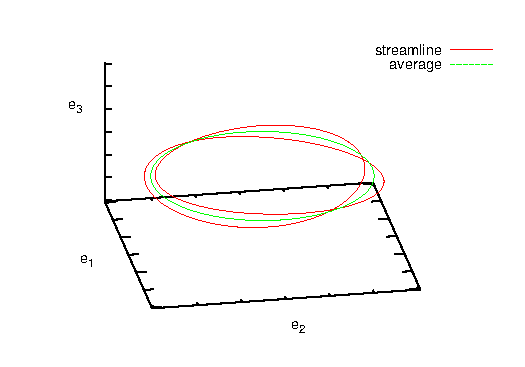
\includegraphics{trefoil_knot.pdf}
%  \caption{
%    A possible streamline (red) with its averaged rotation in green.
%    The streamline was chosen to be a trefoil knot. The reasons for the non-trivial topology are discussed in the text.
%    }
%    \label{fig:particle}
% \end{figure}

\subsection{Interactions between spinless charges}\label{sec:spinless}
When an acoustic charge has no spin (or the spin is ignored)
the equations of motion can be derived from the manifestly gauge invariant energy momentum tensor in  equation \eqnref{TAEM}.
By taking the  divergence and picking out the spatial terms,
the force $\vf$ is found to be \cite{Doran2003}
\begin{align}
  \vf = - \lr{\rho_q\vE + \vJ \times \vB}.
\end{align}
If it is assumed that an acoustic charge $q$ is carried by an `acoustic particle' (a vortex tube without swirl, for instance)
moving at speed $\vu$, then
$\vf = - q\lr{\vE + \vu \times \vB}$, which is the Lorentz force law.
We argue, therefore, that turbulent sources of sound, interact according to the Lorentz-force law when measured acoustically.

Whether this result could be used to model bubble-bubble interactions remains an open question.
% The force law takes the form
% \eqal{
% \dot  u  = - \frac{q}{m_0} F \cdot u
% }{LorentzGA}
% when expressed with geometric algebra, where the dot denotes differentiation 
% with respect to proper time and $m_0$ is the {\em rest mass} of the vortex source,
% presumably the mass  displaced by the differing density of the vortex.


% The divergence of the energy momentum tensor gives the force
% and the spatial component in the lab frame is
% \begin{align}
%   \vf = - \lr{\rho_q\vE + \vJ \times \vB}.
% \end{align}
% If it is assumed that an acoustic charge $q$ is carried by a `particle' moving at speed $\vu$, then
% $\vf = - q\lr{\vE + \vu \times \vB}$, which is the Lorentz force law.
% Turbulent sources of sound, therefore, interact according to the Lorentz-force law when measured acoustically.

%\subsection{Particles with Spin}


\subsection{Other similar studies}

%The  similarities between acoustics and electromagnetism have long been recognised.
By using a relativistic version of Lighthill's formulation of aeroacoustics it was demonstrated 
that the acoustic analogue to the electric field is the Lamb vector (proportional to the Coriolis acceleration),
and that the acoustic analogue to the magnetic field is the vorticity.
%The spacetime vorticity tensor takes the role of the field tensor.
An analogy in this form has been presented before by both Marmanis\cite{Marmanis2000} and Sridhar\cite{Marmanis2000,Sridhar1998}.
However, both these attempts were constructed from Galilean fluid mechanics and so the analogy was only partial.
A complete  analogy, using a relativistic incompressible fluid, was first published by Garrado\cite{Garrado1982} long before the studies of Marmanis and Sridhar.  
Unfortunately, this article was missed by the wider community, 
and has only come to the attention of the author since completing this thesis.
%Nonetheless, the importance of the analogy to ultrasound physics is new.
%To the author's knowledge, the derivation in this report is the first time that the analogy has been  completed.
%The key step, missing in the attempts of Marmanis and Sridhar, 
%is to note that acoustics must be formulated in terms of a Lorentz invariant fluid where
%{\em the speed of sound equals the speed of light}.
%It is only when this step is made that the complete analogy exists for incompressible fluids.
%The motivation for this step is obvious only when it is appreciated that the speed of sound
%may take the role of the speed of light in a relativistic theory.



Relativistic fluids where the sound speed equals the speed of light have been studied many times before
as theoretical curiosities\cite{Taub1978,Pekeris1976, Pekeris1977}.
For example, Pekeris found that Hick's spherical vortex conserves angular momentum if and only if
the sound speed equals the speed of light\cite{Pekeris1977}.
The importance of such fluids, however, has not to the author's knowledge been recognised.
Such fluids represent {\em what can be measured} when distances are obtained by echo-location.
%Acoustics as measured with ultrasound is therefore {\em identical} to electromagnetism as measured with light.
% With hindsight this correspondence is not too surprising.
% For both acoustics as measured with ultrasound and electromagnetism as measured with light 
% attempt to measure the properties of their propagating signal.
% Both, therefore, 
% represent a similarly limited view of the world,
% the limitations manifesting themselves in the linearity of the equations.

An alternative  analogy between acoustics and special relativity is found in the `acoustic analogue gravity' literature (see Barcel{\'o}, Liberati and Visser\cite{Barcelo2005} for a review).
An {\em acoustic} metric is constructed that describes sound carried in bulk flow.
While the description of space and time in this formulation is Euclidean, the acoustic metric turns out to be pseudo-Euclidean,
and therefore obeys the Lorentz transformation.
This results because  sound carried away by a supersonic flow will never reach us
and so the speed of sound is a limiting velocity in transformations.
The analogue gravity literature then goes on to study the gravitational implications of the acoustic metric.
The acoustic metric, albeit Lorentzian, is not the same as Minkowski's metric used here, 
but is a function of the bulk flow.
Analogue gravity does not consider the measurement process and  operates within a world characterised by two metrics, 
the Lorentz invariant acoustic metric
 and the Galilean invariant spacetime  metric.
The correspondence of analogue gravity with relativity theory is therefore partial.
The acoustic analogue to special relativity presented here is complete,
the only difference is that the speed of sound takes the role of the speed of light.


%While the motivations behind the two approaches is similar, in particular the demand that acoustics must be obey a Lorentz invariant metric,
%the approach given here and the approach of analogue gravity are fundamentally different.
%Analogue gravity does not consider the measurement process and so operates within a world characterised by two metrics, 
%the Lorentz invariant acoustic metric (which is a function of the bulk flow)
% and the Galilean invariant spacetime  metric.
%This report argues that only one metric is required;
%the acoustic analogue to special relativity presented here is identical to the original, excepting that is 
%The specPhysics that is measured 
%%Ultrasound measurement demands that the world be described by a Lorentz invariant metric.
%%There is no other way to describe space and time acoustically.
%%In analogue gravity the acoustic metric is Lorentz-invariant, but is not the same as the metric used here.
%%In analogue gravity the metric is a function of the bulk flow,
%%whereas  we argue that this is impossible:
%%the sound speed must be an a priori constant in order to say anything about the world.
%Nevertheless, the success of analogue gravity is very encouraging.
%%Acoustically observed microbubbles could offer an interesting experimental model in this field.




%%% Local Variables: 
%%% mode: latex
%%% TeX-master: "../../tshorrock_thesis"
%%% End: 
